% Document class options:
% =======================
%
% lineno: Adds line numbers.
%
% serif: Sets the body font to be serif. 
%
% twocolumn: Sets the body text in two-column layout. 
% 
%
% Using other bibliography styles:
% =======================
% Not supported at the moment
\documentclass[twocolumn, empirical, authordate, issue]{jote-new-article}


%%% Add the bibliography, make sure it's in the same directory
\addbibresource{horse2.bib}

%%% Add additional packages here if required. Usually not needed, except when doing things with figures and tables, god help you then

% This package is for generating Lorem Ipsum, usage: \lipsum[X] where X is the Xth paragraph of lorem ipsum. OR use [1-5] to generate the first five, etc.

% Fill in the type of article here. Doesn't matter if capitalized. 
%%% Options
% Empirical
% Reflection
% Meta-Research
% Rejected Grant Application
% Editorial

%%% TODO: Make this a 1-5 option scale to reduce the chance of mistyping

% Enter the title, in Title Case Please
% Try to keep it under 3 lines
\jotetitle{The Complexity of Joint Regeneration: How an Advanced Implant Could Fail by Its \textit{In Vivo} Proven Bone Component}

% List abbreviations here, if any. Please note that it is preferred that abbreviations be defined at the first instance they appear in the text, rather than creating an abbreviations list.
%\abbrevs{ABC, a black cat; DEF, doesn't ever fret; GHI, goes home immediately.}

% Include full author names and degrees, when required by the journal.
% Use the \authfn to add symbols for additional footnotes and present addresses, if any. Usually start with 1 for notes about author contributions; then continuing with 2 etc if any author has a different present address.
\author[1\authfn{2}]{Paweena Diloksumpan}
\author[2\authfn{2}]{Florencia Abinzano}
\author[2]{Mylène de Ruijter}
\author[1,2]{Anneloes Mensinga}
\author[1]{Saskia Plomp}
\author[3]{Ilyas Khan}
\author[1]{Harold Brommer}
\author[1]{Ineke Smit}
\author[2]{Miguel Dias Castilho}
\author[1]{P. René van Weeren}
\author[1,2]{Jos Malda}
\author[1,2]{Riccardo Levato}
%Fill it in again for the PDF metadata. Lame workaround but it works
\authorone{Paweena Diloksumpan et al.}

%List the contribution effort here, they will be listed at the end of the page
\contributions{Paweena Diloksumpan and Florencia Abinzano contributed equally to this work.}
%List the acknowledgments. If there is no companion piece, this is listed below the author info
%\acknowledgments{Author Two would like to thank Author One for doing all the work while they could slack off.}
%List possible conflict of interest. Will default to saying no conflict exists.
%\interests{Author One was paid for by Big Failed Experiment}
%List funding
%\funding{}
% Include full affiliation details for all authors
\affil[1]{Department of Clinical Sciences, Faculty of Veterinary Medicine, Utrecht University, 3584 CM, Utrecht, the Netherlands}
\affil[2]{Department of Orthopaedics, University Medical Center Utrecht, Utrecht University, 3584 CX, Utrecht, the Netherlands}
\affil[3]{Center for Nanohealth, Institute of Life Science, College of Medicine, Swansea University, SA2 8PP, Swansea, UK}
% List the correspondence email of the main correspondent
\corraddress{Riccardo Levato, Department of Orthopaedics, University Medical Center Utrecht, Utrecht University, 3584 CX, Utrecht, the Netherlands}
\corremail{\href{mailto:R.Levato-2@umcutrecht.nl}{R.Levato-2@umcutrecht.nl}}

% Optionally list the present address of one of the authors
%\presentadd[\authfn{2}]{Department, Institution, City, State or Province, Postal Code, Country}

% Fill in the DOI of the paper

% Always starts with "10.36850/" and is suffixed with one of the following plus a number
% e  : empirical
% r  : reflection
% mr : meta-research
% rga: rejected grant application
% ed : editorial
\paperdoi{10.36850/e3}

% Include the name of the author that should appear in the running header
\runningauthor{Diloksumpan et al.}

% The name of the Journal
\jname{Journal of Trial \& Error}

% The year that the article is published
\jyear{2021}

%The Volume Number
\jvolume{2}
\jissue{1}
%The website that's listed in the bottom right
\jwebsite{https://www.jtrialerror.com}

%%% Only \paperpublished is necessary, any combination of the other two is possible
\acknowledgments{The authors would like to thank Dr. J.P.A.M. (Thijs) van Loon and Dr. Janny de Grauw for assistance with anesthesia, Dr. S. Veraa for assistance with the radiographic examination, and Paulina Nunez Bernal for assistance with the biomechanical characterization. The authors also wish to acknowledge the funding support from Royal Thai government scholarship (Thailand, PD), the Dutch Arthritis Foundation (LLP-12 and LLP-22), the AO Foundation (Collaborative Research Center AO Foundation, 3D OC Constructs, FA), the European Research Council under grant agreement N0. 647426 (3D-JOINT, JM), and the UK Regenerative Medicine Platform (UKRMP, MR/L02280X/1). The primary antibodies against collagen type II (II-II6B3) developed by T. F. Linsenmayer and E. S. Engvall, respectively, were obtained from the DSHB developed under the auspices of the NICHD and maintained by the University of lowa, Department of Biology, lowa City, IA, USA.}
%When the paper was received
\paperreceived{15 April, 2020}
% When the paper was accepted
\paperaccepted{11 March, 2021}
% When the paper will be published
\paperpublished{23 March, 2021}
\paperpublished{3 March, 2022}
\jpages{}
% When the paper is published but in YYYY-MM-DD format, for the crossmark button
\paperpublisheddate{2021-03-23}
\setcounter{page}{7}
\jpages{7-25}

% The pages of the article, comment out if rolling article
%\jpages{1-12}
% Link to the logo, might be redundant

% Fill something here if this is a rolling/online first article, will make ROLLING ARTICLE show up on the first page

% Sets the paragraph skip to be zero, this should be in the CLS

%%% Companion Piece

% Reflection and Empirical articles have each other as companion pieces. Add the DOI, Title, and Abstract of the respective Companion piece here
\companionurl{https://doi.org/10.36850/r3}
\companiontitle{\newline Nederbragt, H., (2021). Ponies, Joints, Complexity and the Method of Indifference}
\companionabstract{\noindent An important discipline in biomedical science is the repair of damaged organs by in vitro cultured differentaited stem cells. This article evaluates an article in this field, entitled "The complexity of joint regeneration", by Diloksumpan et al. (2021), who described a regeneration experiment of artificial damage of the joint of ponies. The experiment failed an I describe the possible cause of this failure by discussing the design of the experiment in the light of J.S.Mill's Method of Difference, published in 1843. I continue with a discussion of the concept of complexity that was introduced by the authors of the paper, by pointing out that three types of complexity may be distinguished; one of these is complicatedness which characterizes the assumed complexity of the joint experiment. I propose that this complicatedness can be solved by the use of the method of difference.}
\companionkey{Nederbragt2021}

%%% Abstract

% These two set the height and width of the abstract. There's no solution to do this automatically at the moment so fiddle with these a bit. height-width should be 5mm, and ranges between 50-100 are realistic
% Higher number means skinnier abstract
%Enter something here in order for the abstract to disappear. Be sure to also delete the abstract 
% Fill in the keywords that will appear in the abstract, max 7
\keywordsabstract{cartilage, 3D (bio)printing, equine model,
osteochondral, articular cartilage-derived progenitor cells}

%%%%%%%%%%%%%%%%%%%%%%%%%%%%%%%%%%%%%%%%%%%%%%%%%%%
%Document Starts
%%%%%%%%%%%%%%%%%%%%%%%%%%%%%%%%%%%%%%%%%%%%%%%%%%%

\begin{document}
%%% This starts the frontmatter, which includes everything that's on the front page execpt the text of the article
\begin{frontmatter}
\maketitle
%Type your abstract between these things. Max 250 words. Be sure to include the \noindent, looks bad otherwise
\begin{abstract}
     Articular cartilage damage is a major challenge in healthcare due to the lack of long-term repair options. There are several promising regenerative implant-based approaches for the treatment, but the fixation of the implant remains a significant challenge. This study evaluated the potential for repair of an osteochondral implant produced through a novel combined bioprinting-based chondral-bone integration, with and without cells, in an equine model. Implants consisted of a melt electrowritten polycaprolactone (PCL) framework for the chondral compartment, which was firmly integrated with a bone anchor. The bone anchor was produced by extrusion-based printing of a low-temperature setting bioceramic material that had been proven to be effective for osteo-regeneration in an orthotopic, non-load bearing and non-articular site in the same species in an earlier \emph{in vivo} study. Articular cartilage-derived progenitor cells were seeded into the PCL framework and cultured for 28 days \emph{in vitro} in the presence of bone morphogenetic protein-9 (BMP-9), resulting in the formation of abundant extracellular matrix rich in glycosaminoglycans (GAGs) and type II collagen. The constructs were implanted in the stifle joints of Shetland ponies with cell-free scaffolds as controls. Clinical signs were monitored, and progression of healing was observed non-invasively through radiographic examinations and quantitative gait analysis. Biochemical and histological analyses 6 months after implantation revealed minimal deposition of GAGs and type II collagen in the chondral compartment of the defect site for both types of implants. Quantitative micro-computed tomography showed collapse of the bone anchor with low volume of mineralized neo-bone formation in both groups. Histology confirmed that the PCL framework within the chondral compartment was still present. It was concluded that the collapse of the osteal anchor, resulting in loss of the mechanical support of the chondral compartment, strongly affected overall outcome, precluding evaluation of the influence of BMP-9 stimulated cells on \emph{in vivo} cartilage regeneration. 
     \end{abstract}
\end{frontmatter}


\lettrine{L}ocal cartilage damage is a major challenge in human healthcare since it leads to an increased risk of developing early osteoarthritis \parencite{Kloppenburg2020}. Most of the available repair approaches are palliative with limited alleviation time, generating fibrous tissue with reduced mechanical strength \parencite{Kwon2019}. There are no effective treatments that can fully restore the anatomical structure and function of focal cartilage defects. This unmet clinical need drives the ongoing quest for regenerative medicine and tissue-engineering approaches for articular cartilage repair \parencite{Malda2019}.

\begin{companion} \\
\selectfont
H. Nederbragt (2020),\vskip5pt
\textit{Ponies, joints, complexity, and the method of difference}\vskip5pt
{\href{https://doi.org/10.36850/r3}{https://doi.org/10.36850/r3}}
\end{companion}


Many new promising technologies \parencite{Johnstone2019, Patel2019} are currently being developed and tested with the aim of finding an implant that is effective in facilitating regeneration of cartilage. Given the difficulties associated with the fixation of chondral constructs in the joint \parencite{Gotterbarm2008, Mancini2017}, an alternative approach is the use of composite osteochondral constructs composed of distinct osteal and chondral compartments that can be surgically press-fitted into suitably prepared defects, thereby avoiding the risk of dislodgement \parencite{Martin2007}. However, the latter approach still faces many challenges, including design and optimization of the osteal compartment to act as an anchor for the overlying chondral compartment, production of a firm and durable connection between osteal and chondral compartment \parencite{Boushell2017}, and optimization of the composition and structure of the chondral compartment \parencite{Diekman2013, Lee2014}.

\begin{takeHomeMessage}
The collapse of the osteal anchor of these osteochondral implants affected the integration of the construct with the native tissue and seriously compromised the mechanical stability. This precluded drawing firm conclusions about the potential for \emph{in vivo} cartilage repair of the chondral compartment, consisting of bone morphogenetic protein-9 (BMP-9) stimulated progenitor cells. Collapse occurred because bone regeneration competent materials, which had shown success in a different anatomical location, were unable to correctly anchor the implant in the complex biomechanical environment of the joint. The imperfect dimensional match, originating from the intrinsic variability of the 3D printing process, had a much bigger influence than in previous studies. When combined with the brittle nature of the material, the implant was unable to withstand the complex loading of the knee joint.
\end{takeHomeMessage}


To address those challenges, biomaterials that hold the potential for facilitating osteoregeneration within the osteal compartment were recently developed and investigated. First, 3D printed brushite-based scaffolds have been shown to be effective in promoting new bone growth after 6 months in an equine model that used the tuber coxae as implantation site \parencite{VindasBolanos2020}. However, these materials are usually processed using aggressive acidic treatments, precluding the direct incorporation of cells and/or some types of polymer during the fabrication phase. Therefore, an apatite-based scaffold that could harden under physiological conditions into a calcium-deficient hydroxyapatite (CDHA) was developed. This material had been shown to be effective in a 7-month long \emph{in vivo} study, upon implantation in a critical size defect in the tuber coxae of horses. That study was performed to compare two sophisticated architectures with constant and gradient pore size, respectively. The material was shown to facilitate excellent new bone formation, particularly when using the scaffold with constant pore size \parencite{Diloksumpan2020a}. This showed the potential for using such material as an osteal anchor of a tissue-engineered osteochondral graft.

Another major challenge is the connection between the osteal and chondral compartments of the tissue-engineered osteochondral graft when using cell-friendly materials of strongly different mechanical characteristics. Recently, a technique for attaching the chondral compartment to the osteal compartment using melt electrowriting (MEW) was developed \parencite{Diloksumpan2020}, in which MEW fibers of the chondral compartment were partially incorporated into the slowly setting apatite-based osteal compartment, thereby binding the two compartments together. This strategy allows both for optimizing the mechnical properties of the MEW-reinforced chondral compartment, and for integrating the chondral and osteal compartments.

Regarding the seeding of regeneration-competent cells within the chondral compartment, articular cartilage-derived progenitor cells have been recently identified and characterized in both humans and horses as a distinct cell population that has the potential for cartilage repair \parencite{McCarthy2012, Williams2010}. This potential was further shown to be retained in combination with biomaterials \parencite{Frisbie2015, Levato2017}, making this cell type a promising candidate for a comprehensive regenerative approach. Additionally, it was recently discovered that supplementation with BMP-9 during \emph{in vitro} culture of ACPCs resulted in higher expression of gene-markers related with hyaline-like extracellular matrix production, compared to supplementation with transforming growth factor (TGF$\beta$), a more commonly used growth factor in cartilage tissue engineering \parencite{Morgan2020}. This observation sparked interest in further investigation of the potential of BMP-9-stimulated ACPCs for cartilage repair \emph{in vivo}.

The current study aimed at evaluating an osteochondral composite scaffold for cartilage repair. These constructs were composed of a combination of a previously proven osteogenic CDHA 3D printed scaffold for the osteal compartment, onto which a chondral compartment composed by MEW micro-fibrous meshes is tightly anchored. For the chondral compartment, an experimental group in which the MEW structure was seeded with ACPCs that had been stimulated for 28 days with BMP-9 before implantation \parencite{Abinzano2018}, was compared with an implant featuring a non-filled, cell-free MEW cartilage scaffold as control. It was hypothesized that 1) the CDHA scaffold would show comparable performance in the horse when implanted in the subchondral bone as in the tuber coxae in terms of firmly anchoring in the surrounding tissue and inducing bone growth; 2) the novel interface would provide a lasting connection between the osteal and chondral compartments of osteochondral graft; and 3) the engineered chondral compartment of the osteochondral graft containing the stimulated ACPCs would outperform the cell-free structures in terms of \emph{in vivo} cartilage matrix production (specifically, amount and density of type II collagen and GAGs, with resulting mechanical properties as close as possible to those of native, healthy cartilage).

\section{Materials and Methods} 

\subsection{Experimental design} 

To assess the performance of integrated 3D printed osteochondral grafts that contained a cell-laden or a cell-free chondral compartment, the constructs were orthotopically implanted in a large animal model. Eight Shetland ponies (female, age $4-12$ years, weight $149 - 217 kg$ ($166 \pm 29 kg$)) were used and samples were implanted in the medial femoral ridge in the stifle joints. Healing was monitored for 6 months, after which the animals were humanely euthanized. The study was approved by the ethical and animal welfare body of the Utrecht University (Approval nr. AVD108002015307 WP23).

Ponies were housed in individual boxes and fed a limited ration of concentrates together with hay for maintenance and free access to water. Quantitative gait analysis and radiographic examination of the stifle joints were performed before surgery for baseline values. Post-operatively, the animals were kept stabled for 6 weeks with daily monitoring of vital signs, lameness checks at walk, and examination of the operated joints for swelling or other signs of inflammation. In week 5 and 6, they were hand-walked for 10 minutes twice daily and from week 7 on, they were kept at pasture. Quantitative gait analysis and radiographic exams were performed at 3 weeks, 3 months, and 6 months post-operatively. After 6 months, ponies were humanely euthanized for harvesting samples for both quantitative and qualitative analyses. The timeline of the experiment is represented in Figure \ref{fig:figure1}.

\begin{figure*}[t]
\captionsetup{width=\dimexpr\linewidth  +\fullwidthlen\relax}
\begin{adjustwidth}{-\fullwidthlen}{}

 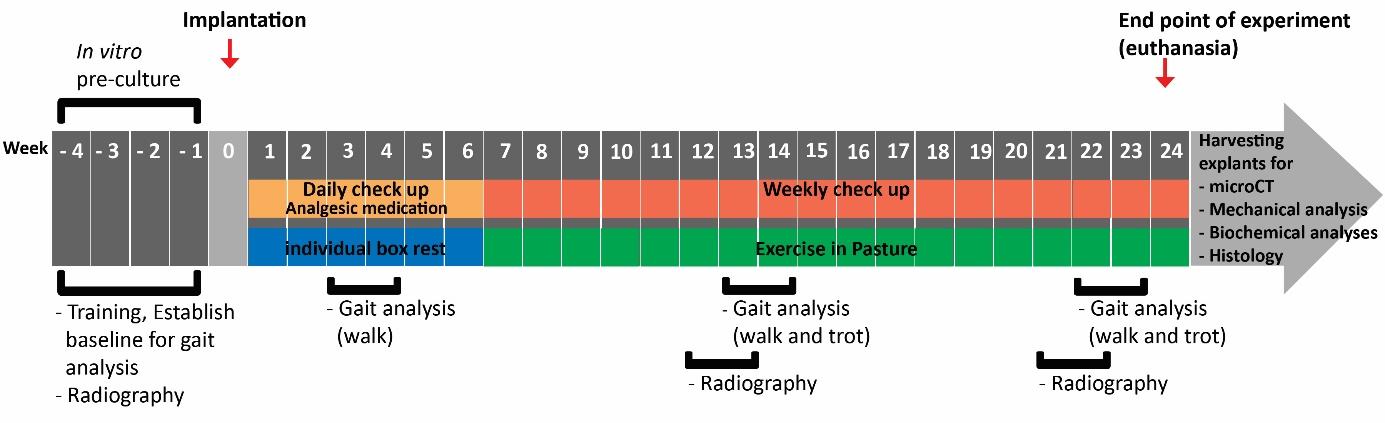
\includegraphics[width=\textwidth+\fullwidthlen]{media/image1.jpg}
 \end{adjustwidth}
 \begin{adjustwidth}{-.5\fullwidthlen}{}
\caption{Flow chart representing timeline of the experiment including health monitoring at each phase of the experiment.}
\label{fig:figure1}

\end{adjustwidth}

\end{figure*}

\subsection{Fabrication of construct} 

Microfiber meshes were produced from medical-grade PCL (Purasorb® PC 12 Corbion PURAC, The Netherlands) by using MEW technology as previously described \parencite{deRuijter2019}. The meshes were produced by horizontally patterning the microfiber (diameter $= 10 \mu m$) to form continuously uniform square spacing ($300x300 \mu m$) and vertically stacking the same pattern until reaching $1300 \mu m$ in total thickness. This structure was achieved by printing with a temperature of 90\textdegree C, a pressure of 1.25 bar, voltage of 10 kV, and collector velocity of $ 15 mm\cdot sec^{-1} $. Additionally, printing was performed at ambient temperature ($22 - 24 \textdegree \text{C}$) with a humidity between $30 - 50\%$. Subsequently, PCL microfiber meshes were hydrolyzed by soaking them in sodium hydroxide (1M NaOH) for 15 minutes and washed in Milli Q water for 10 minutes 4 times. Finally, sterilization was carried out by immersion of the mesh in $70\%$ ethanol for $15$ minutes, followed by air-drying in a sterile cabinet until use.

Printable calcium phosphate (PCaP) paste was prepared as earlier described \parencite{Diloksumpan2020}. In short, $2.2 g\cdot ml^{-1}$ of alpha-tri calcium phosphate ($\alpha$-TCP, average particle size $= 3.83 \mu m$, Cambioceramics, Leiden, the Netherlands) and $0.13 g\cdot ml^{-1}$ of nano-hydroxyapatite (nano-HA, particle size $=200 nm$, Ca\textsubscript{5}(OH)(PO\textsubscript{4})\textsubscript{3}, Sigma-Aldrich) were mixed with $40\% w\cdot v^{-1}$ poloxamer solution (Pluronic® F-127, Sigma-Aldrich). $\alpha$-TCP and nano-HA powder were disinfected with UV-light for 1 hour before mixing. The poloxamer solution was disinfected by filtration through a $0.22 \mu m$ sterile filter (Millex®-GS). This paste was loaded to a cartridge and kept at $4\textdegree \text{C}$ until use.

Osteochondral constructs were produced by combining the PCL microfiber mesh and the PCaP paste to form the reinforcement of the chondral compartment and the biomimetic bone compartment, respectively. Fabrication was performed by directly depositing the PCaP paste (approximated strand diameter $= 250 \mu m$) onto the hydrolyzed MEW mesh (Figure \ref{fig:figure2}). Eighty percent of the mesh thickness was set as the initial height for depositing the first of non-macroporous PCaP layer, as this proved to be the height that did not damage the mesh structure and ensured an optimal integration between the bone compartment and the chondral compartment. The first two layers of PCaP were deposited without macro-spacing, to mimic the subchondral bone plate, and followed by layers with designed macro-spacing of $700 \mu m$ to mimic the cancellous bone section (diameter $= 6 mm$, height $= 5 mm$).

After finishing the fabrication process, the osteochondral constructs were allowed to set at 37\textdegree C under saturated relative humidity to form a solid, biomimetic bone compartment through conversion of the PCaP composite to CDHA. Finally, the osteochondral constructs were disinfected in $70\%$ ethanol and exposed to UV-light for $1$ hour, prior to seeding of cells.

\begin{figure}[t!]
\captionsetup{width=\dimexpr \linewidth + \fullwidthlen\relax}
\begin{adjustwidth}{-\fullwidthlen}{}
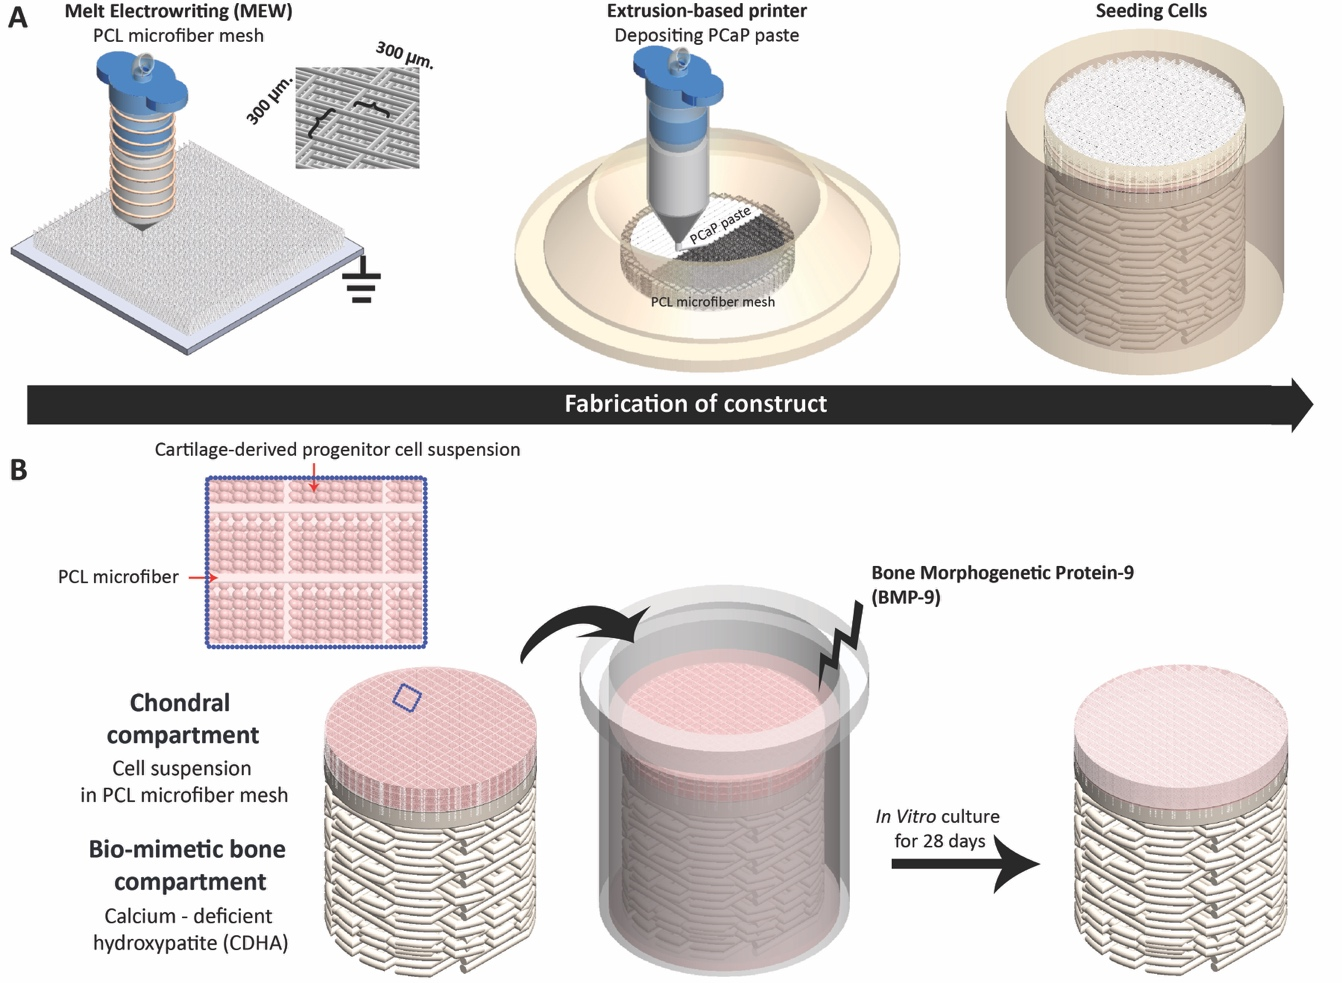
\includegraphics[width=\linewidth]{media/image2.jpg}
\end{adjustwidth}
\begin{adjustwidth}{-.5\fullwidthlen}{}

\caption{Schematic picture representing the fabrication process of the tissue engineered osteochondral constructs.\\ \emph{Fabrication techniques and processes for forming osteochondral graft (A),\\ Material composition of osteochondral graft and process during in vitro preculture (B).}}
\label{fig:figure2}
\end{adjustwidth}
\end{figure}
\subsection{In Vitro pre-culture} 

Allogeneic articular cartilage progenitor cells (ACPCs) were obtained as previously described \parencite{Levato2017, Williams2010} from animals that were euthanized at the Utrecht University Veterinary Hospital for causes unrelated to disease or impairment of the musculoskeletal system and whose remains were donated for research purposes. Briefly, hyaline cartilage was collected in a sterile fashion, minced, and digested at $37\textdegree \text{C}$ with $0.2\% w\cdot v^{-1}$ pronase solution for $2$ hours, followed by $12$ hours in $0.075\%
w\cdot v^{-1}$ collagenase solution. ACPCs were then selected using a fibronectin adhesion assay \parencite{Levato2017}. Cells were expanded in culture and stored in liquid nitrogen until further use. After thawing, cells were expanded until passage 3 prior to their use for the experiment.

The constructs made of the combined CDHA and MEW meshes were disinfected in ethanol and exposed to UV-light for 1 hour as mentioned above. To avoid any pH changes that might affect the cells, the constructs were subsequently washed 3 times for 10 minutes with PBS and then immersed for 1 week in cell culture medium consisting of Dulbecco's Modified Eagle Medium/Nutrient Mixture F-12 (DMEM/F-12, 11320033, Gibco, The Netherlands) supplemented with $10\% v\cdot v^{-1}$
heat-inactivated fetal calf serum (FCS, Gibco, The Netherlands), $0.2 mM$ L-ascorbic acid 2-phosphate (Sigma), $1\%$ MEM Non-Essential Amino Acids Solution (11140035, Gibco, The Netherlands) and $100 U\cdot mL^{-1}$ penicillin with $100 \mu g\cdot mL^{-1}$
streptomycin (Life Technologies, The Netherlands). Media were refreshed every 2-3 days.

On the day of seeding, medium was refreshed 2 hours before seeding and scaffolds were placed inside a custom-made polydimethylsiloxane (PDMS) ring (Figure \ref{fig:figure2}) that prevented overflow of the cell suspension from the cartilage compartment to the bone scaffold. Ten million cells were suspended in $100 \mu l$ of medium and seeded on top of the constructs. The cell suspension was left to settle at the bottom of the cartilage part for 30 minutes. Afterwards, $2 ml$ of cartilage medium supplemented with $ 100 ng\cdot ml^{-1} $ of BMP-9 (PeproTech, The Netherlands) was carefully added to the well. The seeded constructs were cultured for 4 weeks prior to implantation, refreshing the medium 3 times a week.




\subsection{Surgical procedure} 


Ponies were premedicated with detomidine (intravenous (IV), $ 10 \mu g\cdot kg^{-1} $) and morphine (IV,  $0.1 mg\cdot kg^{-1} $) and anesthesia was induced with midazolam (IV, $ 0.06 mg\cdot kg^{-1} $) and ketamine (IV, $ 2.2 mg\cdot kg^{-1} $). Anesthesia was maintained with isoflurane in oxygen together with continuous rate infusion of detomidine (IV, $ 10 \mu g\cdot kg^{-1} $/h) and ketamine (IV, $ 0.5 mg\cdot kg^{-1} $/h). Meloxicam (IV, $ 0.6 mg\cdot kg^{-1} $), morphine (epidural injection, $0.1 - 0.2 mg\cdot kg^{-1} $) and ampicillin (IV, $10 - 15 mg\cdot kg^{-1} $) were administered pre-operatively as analgesic medication and antibacterial preventative therapy, respectively.

The medial femoral ridge of the stifle joint was exposed by arthrotomy and an osteochondral lesion (diameter $= 6 mm$, depth $= 6 mm$) was surgically created using a power drill. The surgical area was flushed by saline for cooling and removal of debris. Cell-laden constructs were implanted press-fit in a randomly chosen hind limb, with the cell-free control being implanted in the contralateral limb. After closing the arthrotomy wound in four layers in routine fashion, procaine penicillin was administered (Procapen, intramuscular (IM), $ 20 mg\cdot kg^{-1} $). Post-operatively, nonsteroidal anti-inflammatory medication (metacam, per os (PO), SID, $ 0.6 mg\cdot kg^{-1} $) was administered for 5 days and opioids (tramadol, PO, BID, $5 mg\cdot kg\textsuperscript{-1}$) were administered for $2$ days.

\begin{figure}[b!]
\captionsetup{width=\dimexpr \linewidth + \fullwidthlen\relax}
\begin{adjustwidth}{-\fullwidthlen}{}
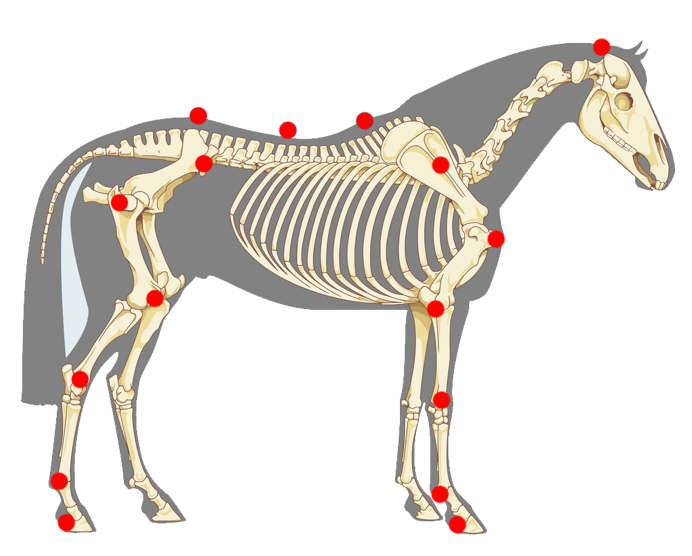
\includegraphics[width=.95\linewidth]{media/image3.png}
\end{adjustwidth}
\begin{adjustwidth}{-.5\fullwidthlen}{}
\caption{\emph{Schematic picture representing location of the markers for gait analysis.}}
\label{fig:figure3}
\end{adjustwidth} 
\end{figure}
\subsection{Gait analysis} 

The ponies were trained on a treadmill prior to the study using a standard protocol for treadmill habituation. Twenty-eight spherical reflective markers with a diameter of $24 mm$ (topline) and $19 mm$ (elsewhere) were attached with double-sided tape and second glue to anatomical landmarks (Figure \ref{fig:figure3}). Kinematic data were collected on a treadmill (Mustang, Fahrwangen, Switzerland) at trot using six infrared optical motion capture cameras (ProReflex, Qualisys, Gothenburg, Sweden) recording at a frame rate of $200 Hz$ for $30$ seconds at each session to obtain a sufficient number of strides.

To process the data, the reconstruction of three-dimensional coordinates of each marker was automatically calculated by Q-Track software (Qtrack, Qualisys, Gothenburg, Sweden). Each marker was identified and labelled using an automated model (AIM model) and manual tracking. Raw data of the designated markers were exported to Matlab (version 2018a, Niantics, California) for further analysis using custom written scripts. For each stride, two symmetry parameters were calculated using the vertical displacement of the head and pelvis (tubera sacrale) markers. For each stride, the differences between the two vertical displacement minima of the head (MinDiffhead) and pelvis (MinDiffpelvis) were calculated. Using the markers, limb-segments were formed and angles between these limb-segments were calculated. The difference between the maximal and minimal angle was defined as the range of motion (ROM) of a joint. For each timepoint, the mean value of all strides for each parameter was calculated.



\subsection{Radiographic examination} 

Stifles were radiographed in 3 projections: lateromedial, craniolateral-caudomedial oblique and caudo-cranial projection using standard machine settings before surgery (baseline), at 3 weeks postoperatively and at 6 months, just before euthanasia.

\subsection{Euthanasia and sample harvest} 

After 6 months, animals were euthanized by induction with Midazolam (IV, $0.06mg\cdot kg\textsuperscript{-1}$ body weight) with ketamine IV, ($ 2.2 mg\cdot kg^{-1} $ body weight) and subsequent administration of sodium pentobarbital (IV, $ 1400 mg\cdot kg^{-1} $ body weight). Next, the stifle joint was exposed, and gross assessment of the medial trochlear ridge was performed, focusing on the degree of filling of the defect, the integration of repair tissue with the surrounding native tissue and the surface quality of the repair tissue. Subsequently, the entire osteochondral area containing the constructs was harvested for further analyses with the aid of a surgical bone saw. Harvested tissues were initially kept in sterilized PBS for micro-computed tomography (micro-CT) scanning, biomechanical analyses and for collecting tissue from the chondral compartment of the implant for biochemical analyses. After this, all tissues were fixed in 4\% formaldehyde for subsequent histological processing.

\subsection{Biomechanical evaluation} 

The compressive properties of the chondral compartment of the defect site, the adjacent surrounding native cartilage and the more distant surrounding native cartilage ($5 - 10 mm$ from the boundary of the defect) ($N=7$ for cell-laden constructs and $N=7$ for cell-free constructs) were evaluated with a dynamic mechanical analyzer (DMA, DMA Q800, TA instrument) equipped with a custom-size compressing probe (diameter $= 2 mm$). A ramp force of $ 0.250 N\cdot min^{-1} $ was applied until reaching $2.0 N$, to limit the deformation of sample to values below $200 \mu m$. Compression modulus was calculated as the slope of the stress-strain curve in the range between $10-12 \%$ strain.

\subsection{Biochemical evaluation} 

Firstly, biochemical analyses were performed on supplemental pre-implantation constructs ($ N=3 $) that had been prepared in the same batch as the constructs that were later implanted. The chondral compartments of 28-day cultured constructs were removed and freeze-dried. Next, dry samples were digested in papain (Sigma Aldrich) at $60\textdegree \text{C}$ overnight. DNA, sulphated glycosaminoglycan (sGAG), and alkaline phosphatase (ALP) content were quantified by performing the Quan-iT-Picogreen-dsDNA-kit assay (Molecular Probes, Invitrogen, Carlsbad, USA), the dimethylmethylene blue assay (DMMB, Sigma-Aldrich, The Netherlands) and the p-nitrophenyl phosphate assay (SIGMAFAST\texttrademark, Sigma-Aldrich), respectively.

Secondly, tissue fractions that were collected from the chondral compartments of harvested implants ($ N=6 $ for cell-laden constructs, $ N=7 $ for cell-free constructs) were kept at $-80\textdegree \text{C}$, followed by lyophilization. Collagen content was quantified using an hydroxyproline assay (L-Hydroxyproline, Merck KGaA), and the sGAG and DNA quantification was performed as described above.
\begin{figure}[t!]
\captionsetup{width= \dimexpr\linewidth + \fullwidthlen\relax }
\begin{adjustwidth}{-\fullwidthlen}{}
 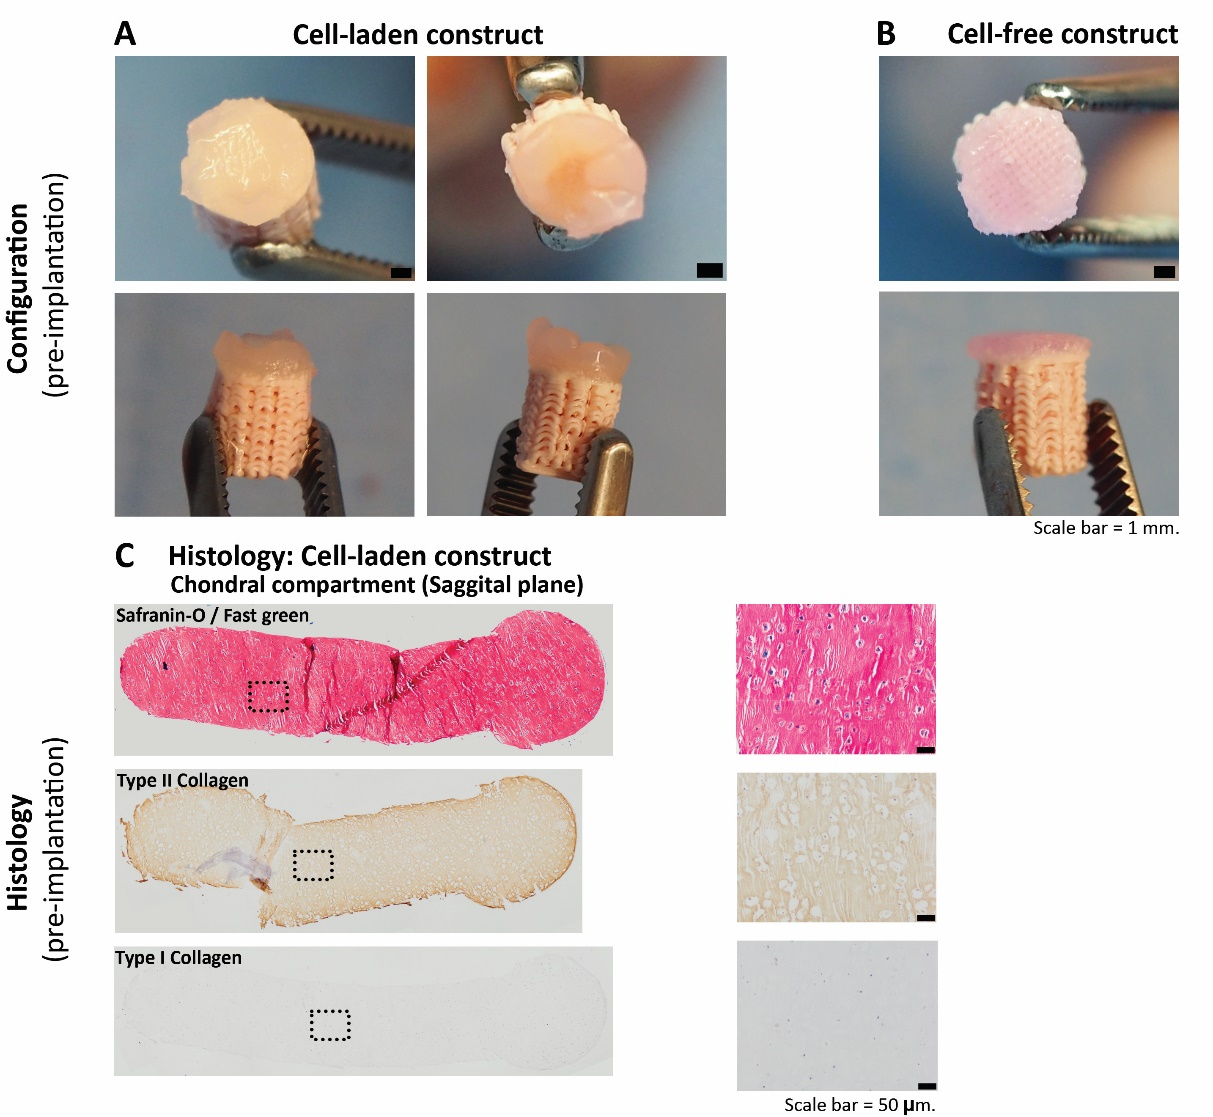
\includegraphics[width=.965\linewidth]{media/image4.jpg}
 \end{adjustwidth}
\begin{adjustwidth}{-0.5\fullwidthlen}{}
\caption{\emph{Representative pictures of cell-laden and cell-free osteochondral constructs at the time of implantation.} Cell-laden (A) and cell-free constructs (B) at the time of implantation. Positive safranin-O staining indicating the presence of glycosaminoglycans (pink = positive), positive type II collagen (brown = positive) and negative type I collagen (brown = positive) immunohistochemistry were observed in the chondral compartment of the cell-laden constructs before implantation (C).}
\label{fig:figure4}
\end{adjustwidth}
\end{figure}
\subsection{Microcomputed tomography} 

Microcomputed tomography was employed for the quantitative analysis of the bone compartments from the harvested osteochondral lesions ($ N=7 $ for cell-laden constructs, $ N=7 $ for cell-free constructs). Six freshly made osteochondral grafts were scanned in a micro-CT scanner (Quantum FX-Perkin Elmer) to quantify the initial volume of PCaP material, pre-operatively. The post-mortem harvested tissue containing the defect area and the surrounding native tissue were similarly scanned (voltage $= 90 kV$, current $= 200 \mu A$, voxel size $= 30 \mu m\textsuperscript{3}$ and total scanning time $= 3 minutes$). Subsequently, the 3D-reconstructed images were processed and analyzed using image J software \parencite{Schindelin2012} and Bone J plugin \parencite{Doube2010}. Two-dimensional regions of interest (ROIs) were selected in an axial plane at the boundary between the defect and the surrounding native tissue and interpolated to form a three-dimensional volume of interest (VOI). Thresholding was performed to separately select areas of ceramics and newly formed bone respectively for further calculation. Then, the percentages of mineralized newly formed bone, of non-mineralized tissue and of remaining ceramics, including the percentage of ceramics volume loss, were quantified.

\subsection{Histological evaluation} 

Firstly, supplemental pre-implantation constructs ($N=3$) that had been prepared in the same batch as the ones that later were implanted were fixed in $4\%$ formaldehyde. After decalcification in $0.5M$ Ethylenediaminetetraacetic acid (EDTA) disodium salt ($pH = 8$) for $1$ day, tissues were dehydrated with graded ethanol series, cleared in xylene, and embedded in paraffin. Paraffin embedded tissues were sliced to $5 \mu m$ sections. Histochemical evaluation of GAG was done by safranin-O / fast green staining. Type I collagen (primary antibody: monoclonal antibody EPR7785, $1.083 mg\cdot ml^{-1}$, Abcam) and type II collagen (primary antibody: monoclonal antibody II-II6B3, $0.06 mg\cdot ml^{-1}$, DSHB) were visualized by immunohistochemistry.

The tissues that were harvested after $6$ months ($N=7$ for cell-laden constructs, $N=7$ for cell-free constructs) were kept in $4\%$ formaldehyde and then decalcified in $0.5M$ EDTA disodium salt ($pH = 8$) for $24$ weeks. Decalcified tissues were cut into two halves before processing to enable visual inspection of the center of the lesion. Tissues were dehydrated with graded ethanol series, cleared in xylene and finally embedded in paraffin. Paraffin embedded tissues were sliced to $5 \mu m$ sections. For assessment of morphology and cell distribution, hematoxylin-eosin staining (Mayer's haematoxylin, Merck 109249 and eosin, Merck 115935) was performed. GAG and collagen alignment were assessed after safranin-O / fast green and picrosirius red staining, respectively. Types I collagen and type II collagen were visualized by immunohistochemistry, as described above. For immunohistochemistry, all samples were treated according to previously published protocols \parencite{Levato2017}. Stained histological slides were imaged using a light microscope (Olympus BX51, Olympus Nederland B.V.), equipped with a digital camera (Olympus DP73, Olympus Nederland B.V.). To observe the picrosirius red stained slides, a polarizer was also mounted to the light microscope.

\subsection{Statistical analysis} 

Normality of distribution of the data was assessed from skewness, kurtosis, and Q-Q plots. Results were reported as mean $\pm$ standard deviation. Wilcoxon signed rank tests were used to analyze the biochemical, biomechanical, and micro-CT data. Statistical significance was set at $p = 0.05$. All tests were performed using Matlab (version R2018b, The MathWorks, Inc.).

To evaluate the gait parameters, stride-level data were analyzed with R software (version 3.6.0, R Core Team, 2019), using package NLME (version 3.1-137) for mixed modelling. Dependent variables were investigated for normality using normal probability plotting and examining for skewness and kurtosis. If not normally distributed, data were transformed to permit linear mixed modeling. The random effect was subject and timepoint was the fixed effect. Significance was set at p \textless{}
0.05 and p-values were corrected using the false discovery rate method. Residual plots were checked for heteroscedasticity versus the outcome, as well as for normality in Q-Q plots.
\begin{figure}[t!]
\captionsetup{width=\dimexpr \linewidth + \fullwidthlen\relax}
\begin{adjustwidth}{-\fullwidthlen}{}
 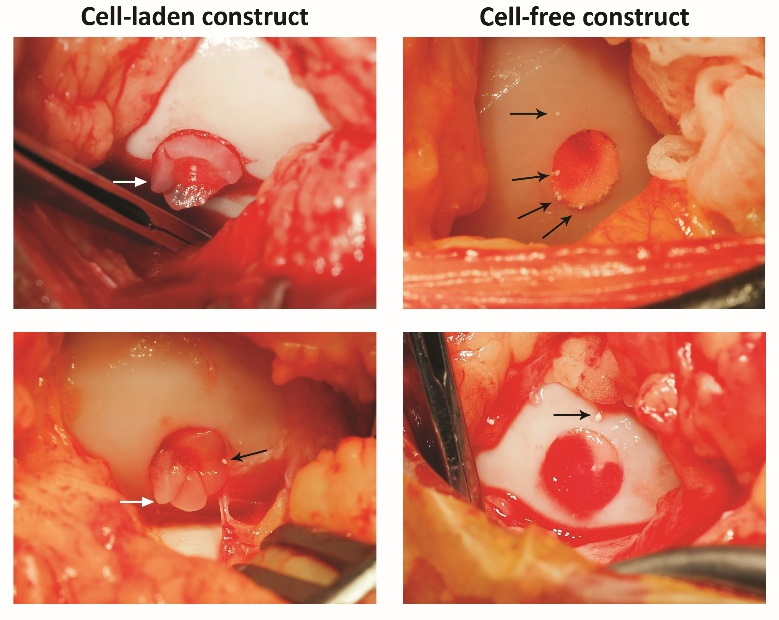
\includegraphics[width=\linewidth]{media/image5.jpg}
 \end{adjustwidth}
 \begin{adjustwidth}{-.5\fullwidthlen}{}
\caption{\emph{Representative pictures show white fragments of broken ceramic after press-fitting cell-laden and cell-free osteochondral constructs into the defect.} Black arrows indicate the position of some visible bioceramic fragments. White arrows indicate protrusion of the chondral compartment}
\label{fig:figure5}
\end{adjustwidth}
\vskip-.5\baselineskip
\end{figure}
\section{Results} 

\subsection{In vitro} 

After 4 weeks of preculture, macroscopic characterization of tissue formation and hyaline-like extracellular matrix production were assessed both quantitatively and qualitatively within the chondral compartment of the cell-laden osteochondral constructs. The BMP-9 stimulated ACPCs meant to colonize the MEW scaffolds formed neo-tissue that had grown into a disc shape after 3 weeks of culture. During the 4\textsuperscript{th} week of culture, outgrowth from the MEW meshes was observed (Figure \ref{fig:figure4}A) from this construct. Cell-free constructs did not change after immersion in growth factor-free medium for 4 weeks (Figure \ref{fig:figure4}B). Biochemical analyses of the chondral compartment of the cell-laden constructs were performed to quantify matrix production of stimulated cells toward chondrogenic lineage and osteogenic lineage, which revealed the presence of GAGs (GAGs$\cdot$ DNA\textsuperscript{-1} was $199.7 \pm 67.7 \mu g\cdot \mu g^{-1}$) and ALP activity (ALP·DNA\textsuperscript{-1} was $3702 \pm 2111 U\cdot\mu g^{-1}$), respectively. Safranin-O staining and type II collagen immunohistochemistry were also performed to visualize hyaline-liked matrix production from stimulated cells, which revealed abundant deposition of GAGs and type II collagen within the constructs after 3 weeks of \emph{in vitro} culture (Figure \ref{fig:figure4}C), showing that the chondral compartments of the constructs (meant for subsequent implantation) were filled with a hyaline cartilage-like tissue. No preferential alignment of the collagen fibers could be observed.



\subsection{Evaluation during surgical implantation} 

Both cell-laden and cell-free constructs were press-fit implanted into the surgically created defect sites. During this procedure, the slightly irregular outer edge of the osteal part of the construct hampered easy sliding of the construct down into the defect and some fragmentations of the edges of the bioceramic scaffold was observed during the procedure. This was similar for the cell-laden and cell-free constructs, which had identical osteal parts (Figure \ref{fig:figure5}). Further, of some cell-laden constructs, the surface of the chondral compartment was not level over the entire circumference with the surrounding native cartilage after press-fitting into the defect site.




\subsection{Post-operative clinical monitoring} 

After surgical implantation, the animals were checked clinically for physical appearance and vital signs on a daily basis. All ponies recovered well from anesthesia after surgery and passed uneventfully through the rehabilitation period without any abnormalities in body temperature or behavior, with good weight-bearing on all operated limbs and no clinical signs of lameness during the entire period, with the exception of a single pony that developed severe lameness at 10 weeks after surgery. This pony was treated with anti-inflammatory medication and examined radiographically, which revealed extensive osteolysis around the created lesion. Because of persistent discomfort, the pony was euthanized at 12 weeks after surgery. Therefore, it was excluded from all analyses.

\subsection{Gait analysis} 

Objective gait analysis was used to check for lameness or other signs of dysfunction of the musculoskeletal system. Objective data retrieved before implantation and at the end of the experiment were assessed for relevant parameters, including symmetry parameters and limb parameters.
\begin{figure*}[t!]
 \begin{adjustwidth}{-\fullwidthlen}{}

 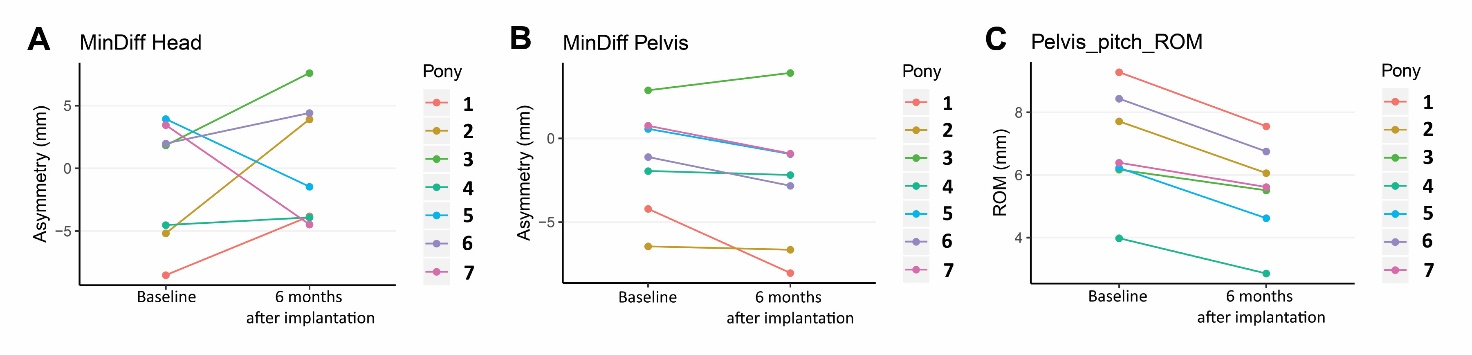
\includegraphics[width=\textwidth +\fullwidthlen]{media/image6.jpg}

\caption{\emph{Gait analysis: Symmetry parameters. \textit{Symmetry data of the head (A) and pelvis (B) show no consistent differences over time. However, pelvis pitch decreased consistently in all individuals (C).}}}

\label{fig:figure6}
 \end{adjustwidth}
\end{figure*}

\begin{figure}[b!]
\captionsetup{width=\dimexpr\linewidth+\fullwidthlen\relax}
\begin{adjustwidth}{-\fullwidthlen}{}

\centering 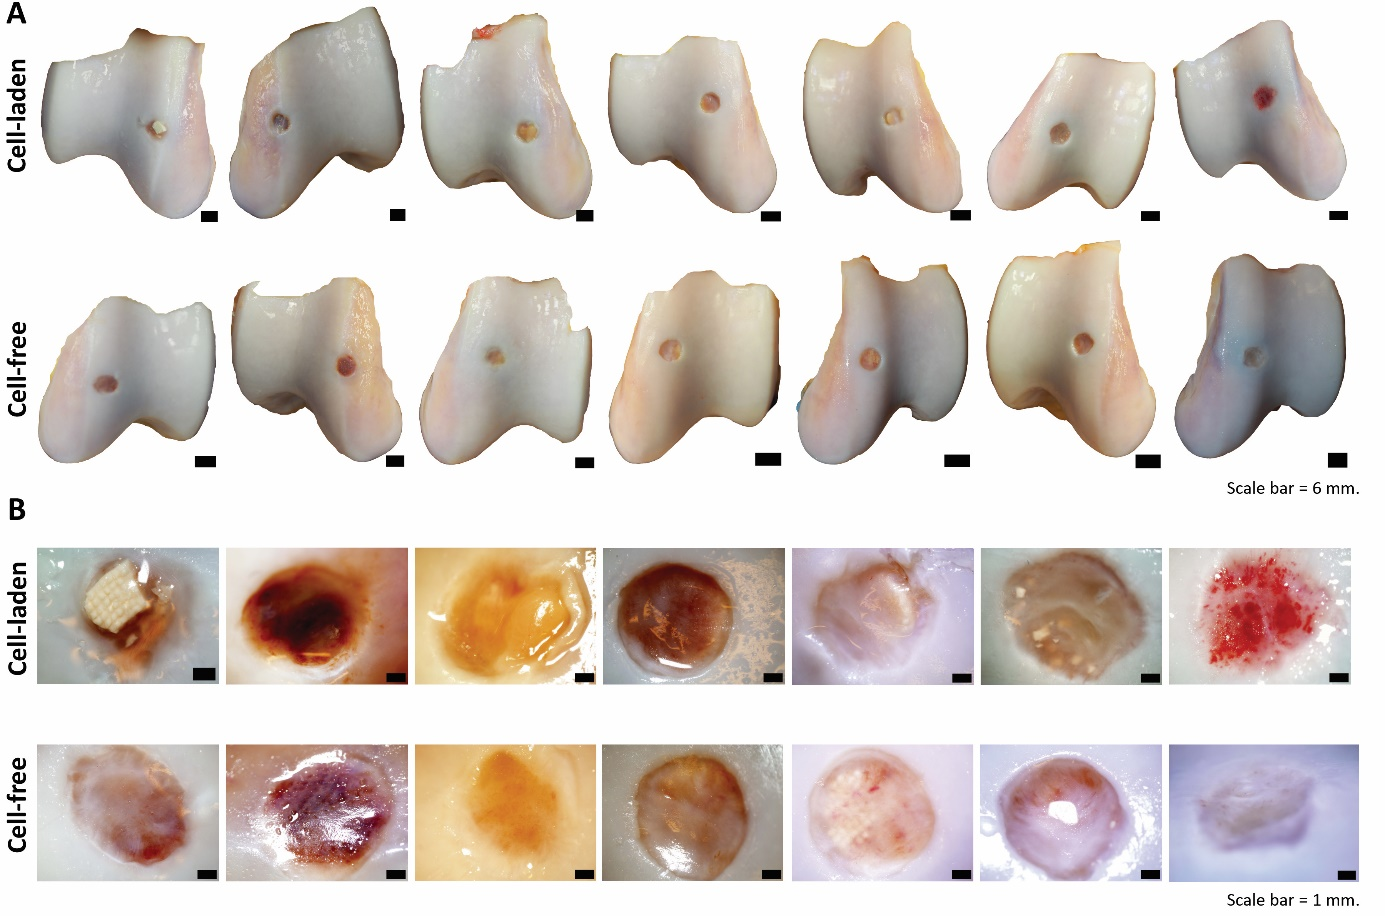
\includegraphics[width=\columnwidth+\fullwidthlen]{media/image7.jpg}
\end{adjustwidth}

\begin{adjustwidth}{-.5\fullwidthlen}{}
\caption{\emph{Macroscopic appearance of the repair tissue and surrounding native tissue in all individual animals at euthanasia.} Macroscopic appearance of the defect site and surrounding femoral ridge (A). Close-ups of macroscopic appearance at the defect site (B).}
\label{fig:figure7}
\end{adjustwidth}

\end{figure}
\subsubsection{Symmetry parameters} 

Front and hind limb lameness were analyzed through evaluation of the symmetry parameters of the head (MinDiff Head (Figure \ref{fig:figure6}A)) and of the pelvis (MinDiff Pelvis (Figure \ref{fig:figure6}B)). These values reflect the differences in minimal vertical displacement with a negative MinDiff indicating a left-sided asymmetry and a positive MinDiff a right-sided asymmetry. In the treated ponies (except for the case referred to above that was euthanized), for both the head and the pelvis, there was no clear pattern in the direction of the asymmetries between baseline and endpoint and those differences between baseline and endpoint were minimal and statistically not significant. Therefore, symmetry measures could not discriminate between cell-laden and cell-free constructs. Further, there was also no clear effect of timepoint on pelvis roll and pelvis yaw range of motion (Supplementary Figure \ref{fig:sup1}), however, pelvis pitch range of motion (ROM) (Figure \ref{fig:figure6}C) decreased for all subjects with almost 20\% over time (Supplementary Table \ref{tab:table1}).


\subsubsection{Limb parameters, effects of time} 

There was a significant effect of time for the height the toe was lifted from the surface during the swing phase of the limb that decreased significantly in the cell-free treated limbs, but not in the limbs treated with cell-laden constructs (Supplementary Table \ref{tab:table1}). The only other significant effect of time was a decrease in the extension of the metacarpophalangeal joint of the forelimb ipsilateral to the hind limb that had been treated with cell-laden constructs, indicating unloading of that forelimb (Supplementary Table \ref{tab:table1}).

\subsubsection{Limb parameters, differences between cell-laden and cell-free at endpoint} 

There were no significant differences between any of the cell-laden and cell-free limb parameters at the end of the experiment. Results from the linear mixed model are shown in Supplementary Table \ref{tab:table2}.


\subsection{Radiographic examination} 

Healing progression within the osteal compartment of the implanted osteochondral constructs was followed up non-invasively through radiographic examination. On the radiographs taken at baseline, 3, and 6 months, no obvious abnormalities in term of the architecture of the surrounding native tissue were detected, other than the defects that had been created. This was with the exception of the pony that developed severe lameness. In that animal, severe osteolysis was noted at the implantation site 3 months after the implantation (Supplementary Figure \ref{fig:sup2}).
\begin{figure}[t!]


\captionsetup{width=\dimexpr \linewidth + \fullwidthlen\relax}

\begin{adjustwidth}{-\fullwidthlen}{}
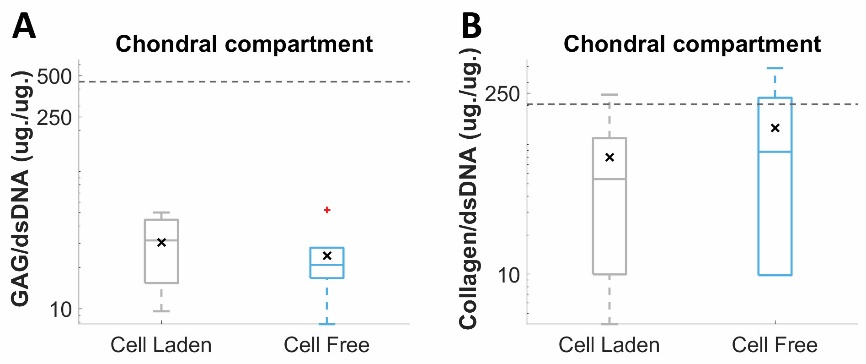
\includegraphics[width=\columnwidth+\fullwidthlen]{media/image8.jpg}

\end{adjustwidth}
\begin{adjustwidth}{-.5\fullwidthlen}{}

\caption{\emph{Biochemical analysis from chondral compartment at the defect site after an implantation for 6 months.} Quantitative analysis of GAG·DNA\textsuperscript{-1} between cell-laden and cell-free treatments (A). Quantitative analysis of collagen$\cdot$ DNA\textsuperscript{-1} between cell-laden and cell-free treatments (B) ($x$ = mean). Grey dotted line indicates level in native cartilage.}
\label{fig:figure8}
\end{adjustwidth}
\end{figure}



\begin{figure}[h!]
\captionsetup{width=\dimexpr \linewidth + \fullwidthlen\relax}

\begin{adjustwidth}{-\fullwidthlen}{}
 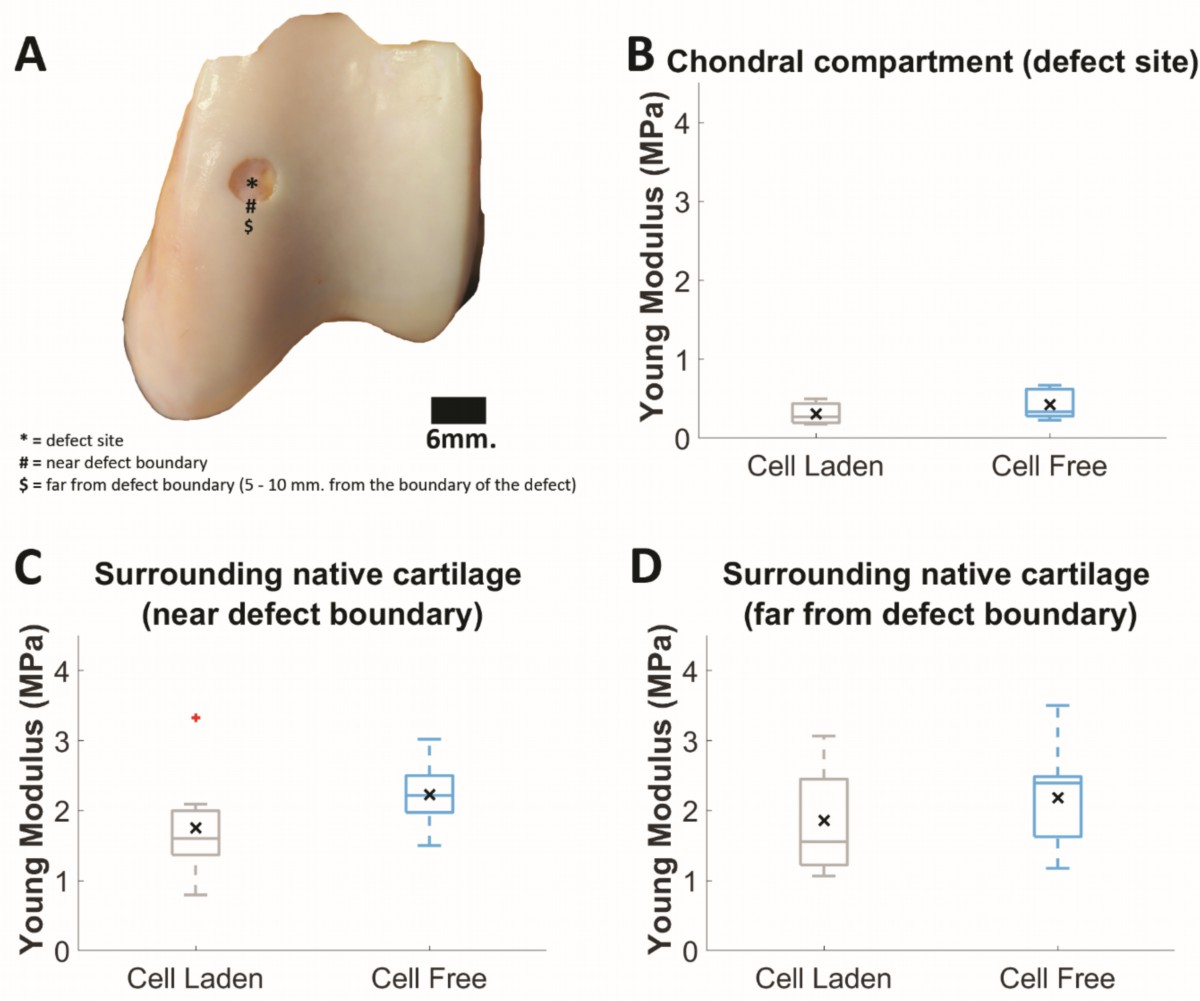
\includegraphics[width=.95\linewidth]{media/image9.jpg}
\end{adjustwidth}

\begin{adjustwidth}{-.5\fullwidthlen}{}
\caption{\emph{Compression modulus of the chondral compartment at the defect site and surrounding native cartilage of harvested samples 6 months after implantation.} Schematic picture demonstrating locations where mechanical properties were analyzed (A). Compression modulus of the chondral compartment of cell-laden and cell-free constructs at 6 months (B) and at two sites of the native cartilage, close to the border of the defect (C) and further away (D). ($x$ = mean).}
\label{fig:figure9}
\end{adjustwidth}
\vskip-.9\smallwidth
\end{figure}


\subsection{Post-mortem macroscopic evaluation of the repair tissue} 

Macroscopic characteristics, for instance, color, appearance, and filling level of the lesion, were observed and documented before harvesting tissue sample for further analyses. After 6 months, macroscopic evaluation revealed that the defects were filled with repair tissue that in all cases did not fill the entire defect and remained lower than the level of the surrounding native cartilage in both cell-laden and cell-free treatments (Figure \ref{fig:figure7}A). The color of the repair tissue was variable (from reddish, to yellow and translucent) within the different treatments (Figure \ref{fig:figure7}B). In some cases, ceramic fragments could be observed within the repair tissue of the chondral compartment.




\subsection{Biochemical analyses of repair tissue within the chondral compartment} 

The deposition of GAGs and collagen, the two main elements that compose cartilage extracellular matrix, were quantified within the chondral compartment of the osteochondral graft 6 months after implantation. There were no significant differences in either GAGs (cell-laden: $30.46 \pm 15.95 \mu g\cdot\mu g^{-1}$, cell-free: $24.44 \pm 15.31 \mu g\cdot g^{-1}$) or collagen expressed per DNA (cell-laden: $79.66 \pm 91.21 \mu g\cdot\mu g^{-1}$, cell-free: $134.21\pm 153.73 \mu g\cdot\mu g^{-1}$) between the chondral compartments of the cell-laden and cell-free constructs (Figure \ref{fig:figure8}A, 8B and Supplementary Figure \ref{fig:sup3}). However, all values were substantially lower than those from native cartilage (Figure \ref{fig:figure8}, grey dotted line) that was harvested distantly from the defect site.


\subsection{Biomechanical properties of the repair tissue within the chondral compartment} 

Compressive strength of the chondral compartment was assessed and compared in three different locations: the defect site, adjacent surrounding native tissue, and distant surrounding native tissue (Figure \ref{fig:figure9}A), the latter two as control measurements from healthy cartilage tissue. There were no significant differences in the Young's modulus of the chondral compartment between cell-laden ($0.31 \pm 0.13 MPa$) and cell-free ($0.42 \pm 0.19 MPa$) constructs (Figure \ref{fig:figure9}B). This was also true for two sites of the native cartilage, one close to the border of the defect (cell-laden: $1.75 \pm 0.80 MPa$, cell-free: $2.22 \pm 0.48 MPa$) and one at $5 - 10 mm$ from the defect boundary (cell-laden: $1.86 \pm 0.78 MPa$, cell-free: $2.19 \pm 0.77 MPa$) (Figure \ref{fig:figure9}C, 9D). However, the compression modulus of the native tissue was substantially higher (approximately $5-6$-fold) than inside the chondral compartment of the implant.




\subsection{Micro-CT evaluation of repair tissue within the osteal compartment} 

Bone healing and integration after was assessed through micro-CT scanning 6 months after implantation. Micro-CT images showed significant bone loss surrounding the implant in both the cell-laden and the cell-free groups, which could be visualized as black areas between the porous bioceramic structure (white) and the surrounding native bone (grey). However, mineralized bone formation could be visualized in some scaffolds from both groups with an integration to neighboring native bone (Figure \ref{fig:figure10}A). Statistically, there were no significant differences in mineralized bone formation (cell-laden: $6.14\% \pm 10.09\%$, cell-free: $4.73\% \pm 4.93\%$) and non-mineralized tissue (cell-laden:  $ 81.38\% \pm 15.37\% $, cell-free:  $ 74.71\% \pm 12.44\%$). However, there was a significant difference in the amount of remaining ceramics between the two groups (cell-laden:  $ 12.48\% \pm 9.75\% $, cell-free:  $ 20.56\% \pm 10.54\% $($p = 0.0313$)) (Figure \ref{fig:figure10}B). In line with this, there was a difference in the degradation of ceramics in the cell-laden construct versus the cell-free constructs (cell-laden:  $ 79.02 \pm 16.18 \% $, cell-free:  $ 63.20 \pm 13.90 \% $($p = 0.0313$)) (Figure \ref{fig:figure10}C).

\begin{figure*}[t!]
\captionsetup{width=\dimexpr \linewidth + \fullwidthlen\relax}

\begin{adjustwidth}{-\fullwidthlen}{}
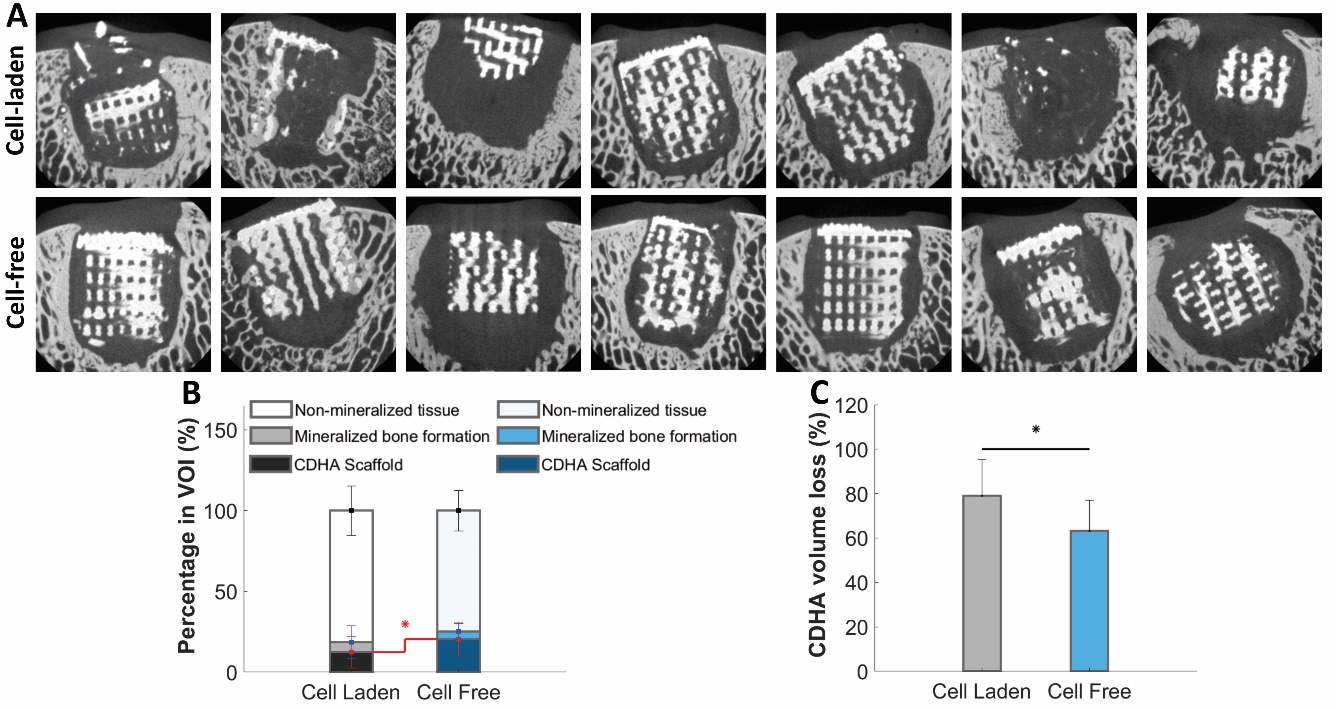
\includegraphics[width=\textwidth+\fullwidthlen]{media/image10.jpg}
\end{adjustwidth}
\begin{adjustwidth}{-.5\fullwidthlen}{}

\caption{\emph{Representative micro-CT images from the middle of the sagittal plane of the constructs and quantification from 3D-reconstruction of micro-CT.} Representative micro-CT images from the middle of the sagittal plane of the constructs (white = ceramics, grey = mineralized tissue, black = non-mineralized tissue) (A). Quantitative analysis from micro-CT reconstruction showing percentage of mineralized bone formation, non-mineralized tissue, and remaining ceramics (B). The volume loss of ceramics was slightly higher in the cell-laden constructs compared to the cell-free ones (C).}
\label{fig:figure10}
\end{adjustwidth}
\end{figure*}

\subsection{Histological evaluation of the osteochondral repair tissue} 

Histological slides were assessed to identify the composition of the repair tissue matrix deposited within the defect site. In the chondral compartment, the defect sites of both cell-laden and cell-free structures were filled with fibrous repair tissue with degenerated and necrotic superficial surface with minimal inflammatory reaction, as revealed by H\&E and safranin-O staining (Figure \ref{fig:figure11}, Supplementary Figure \ref{fig:sup4}, Supplementary Figure \ref{fig:sup6}, and Supplementary Figure \ref{fig:sup7}). Integration at the boundary of the defect between chondral repair tissue and surrounding native cartilage was observed in both groups. The production of GAGs, type II collagen, and type I collagen was very limited in the repair tissue in both groups (Figure \ref{fig:figure11}). The organization of the collagen fibrils in both groups seemed random, without any hierarchical pattern that could be identified by polarized light imaging of picrosirius red staining. Additionally, the special distribution of PCL-microfibers, which had disappeared because of the xylene treatment during sample preparation, was still traceable within the chondral compartment of both groups (1 out of 7 for cell-laden and 5 out of 7 for cell-free structure).

In the bone compartment, there was positive staining for type I collagen in some scaffolds from both groups at places where there were islands of new mineralized bone formation. There were multifocal coalescing spots of inflammatory reaction characterized by macrophages, multinucleated giant cells, lymphocytes, eosinophils, and plasma cells (Supplementary Figure \ref{fig:sup5}, Supplementary Figure \ref{fig:sup6}, Supplementary Figure \ref{fig:sup7}).

\begin{figure*}[b!]
\captionsetup{width=\dimexpr\textwidth+\fullwidthlen\relax}
\begin{adjustwidth}{-\fullwidthlen}{}
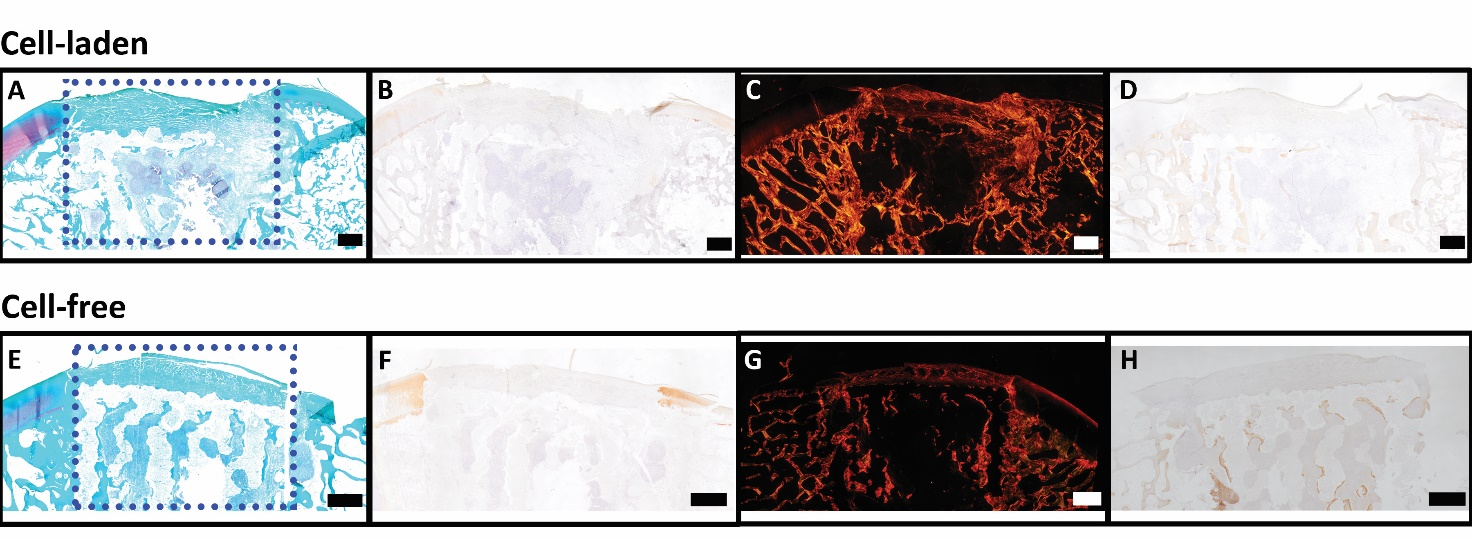
\includegraphics[width=\textwidth+\fullwidthlen]{media/image11.jpg}
\end{adjustwidth}
\begin{adjustwidth}{-.5\fullwidthlen}{}
\caption{\emph{Representative histological images from the center part of cell-laden and cell-free structures after implantation for 6 months.} Safranin-O/fast green (red color = positive) (A, E); Collagen type II (brown color = positive) (B, F); Picrosirius-red (C, G); collagen type I (brown color = positive) (D, H) of cell-laden (A-D) and cell-free structures (Scale bar = $1mm$).}
\label{fig:figure11}
\end{adjustwidth}
\end{figure*}


\section{Discussion} 

This study aimed to evaluate the efficacy of an engineered osteochondral composite scaffold that was fabricated by combining a proven osteogenic CDHA scaffold for the osteal compartment with a novel interface for the connection between the chondral and osteal compartments. For the chondral compartment, BMP-9 stimulated cell-laden and cell-free constructs were compared. The cell-laden constructs contained \emph{in vitro} formed tissue that was rich in GAGs and type II collagen, obtained by seeding Articular Cartilage Progenitor Cells (ACPCs) and stimulating them with BMP-9 for 4 weeks prior to implantation. After implantation in an equine osteochondral defect for 6 months, there was poor chondral repair tissue in both the cell-laden and cell-free implants. The repair tissue was akin to fibrocartilage and was characterized by the presence of fibrous tissue with low content of GAGs and type II collagen and a degenerated surface. The CDHA scaffold had failed to act as an osteal anchor, as evidenced by the radiographical images showing misalignment and partial collapse of the CDHA construct, the presence of CDHA fragments within the defect and in the surrounding tissues, and a limited volume of newly formed calcified bone in the pores of the osteal anchor.

In the quest for a method to achieve satisfactory and durable repair of articular cartilage, several osteochondral grafts that incorporate cells and that were manipulated to optimize biochemical and biomechanical properties, have been investigated in the past decades \parencite{Huang2016}. Articular Cartilage Progenitor Cells have become a promising cell source due to their ability to retain their chondrogenicity after their expansion for several passages \parencite{Williams2010}. Recently, growth factor BMP-9 was shown to be a potent stimulator of chondrogenic differentiation of this cell type \emph{in vitro} \parencite{Morgan2020}. This warranted further investigations to evaluate the use of BMP-9 stimulated ACPCs for cartilage repair \emph{in vivo}. Indeed, the cell-laden chondral compartment showed a high presence of neo-cartilage extracellular matrix production after pre-culture at the time of implantation, yet the average GAG content decreased approximately 6.5-fold during the \emph{in vivo} implantation period. The GAG content of cell-laden constructs in fact decreased to the level of the cell-free constructs, suggesting loss or disintegration of the \emph{in vitro}
formed tissue. Which factor initiated this loss of \emph{in vitro}
formed tissue remains unclear. A previous study from \textcite{McCarthy2012} demonstrated superior results in using ACPCs for cartilage repair in an equine model, in comparison with mesenchymal stem cells. However, due to the use of different materials and cell culture protocols, it is impossible to directly compare those results with the ones from the current study. Several factors might have been involved in the deterioration of the chondral compartment in this study, most prominently mechanical stresses due to the partial failure of the osteal basis and the resulting poor osteointegration \parencite{Heuijerjans2018}.

The nature of the osteal anchor is an important factor when developing tissue-engineered osteochondral implants. Much work has been done on the development of several types of bone grafts and many of these are routinely used in clinical settings \parencite{Oryan2014}, so of the various elements of an osteochondral implant, the bone part is seemingly the least difficult one. However, the relationship between the osteal anchor and the quantity and quality of the repair tissue in the chondral compartment has been the subject of debate \parencite{Bal2010} and it is still unclear what osteal anchor would form the best base for facilitating cartilage repair. The exact same bioceramic material tested in this long-term, orthotopic equine study, had previously been shown to successfully guide osteoregeneration in the same species, when implanted in the tuber coxae, an anatomical locus less subject to intense mechanical loads \parencite{Diloksumpan2020}. Additionally, this previous study also focused on comparing different pore architecture within the 3D printed bone scaffolds. The scaffold architecture that led to the highest rate of new bone formation, consisting of a constant pore size across the sample, was selected for the present study, with the goal of maximizing neo-bone repair \parencite{Diloksumpan2020}. However, there are two major differences with the use of the material in the current study. First, in the previous study the material was implanted in the tuber coxae, which is an orthotopic area but not representative of the intra-articular environment. Second, in the former study the implant was surrounded by a cylindrical case made of PCL that served to prevent bone ingrowth from the sides. Without such a shell of the mechanically deformable PCL in the current study, the surgeon encountered difficulties during the surgical placement of the implants, provoked by the non-resilience and brittleness of the CaP-based material, combined with some deviation from an ideal cylindrical shape of the CDHA implant. This resulted in fragments breaking off from the bioceramic osteal anchor. In fact, although inadvertently and as a side-effect, this problem of fragment formation was avoided in the former study when using PCL to encase. Polycaprolactone is deformable material, and the encasing will have facilitated the sliding of the ceramic implant into the defect. The duration of both studies was not identical (7 months in the earlier study, 6 months in the current), which makes direct comparisons between the two impossible. However, there were clear histological differences with many more multifocal to coalescing inflammatory reactions in both cell-laden and cell-free implants in the current study, compared to the earlier study, in which there were very few inflammatory cells visible. This difference is likely due to the chronic irritation caused by fragments of material and to instability resulting from the imperfect fit of scaffold within the defect in the current study.
\begin{originalPurpose}
The current study aimed at evaluating a cell-laden and a cell-free version of an osteochondral composite scaffold for cartilage repair that consisted of an \emph{in vivo} proven osteogenic bone scaffold for the osteal compartment and made use of a novel interface for the connection of the chondral and osteal compartments.
\end{originalPurpose}

Some scaffolds from the current study collapsed and showed misalignment of the CDHA structure within the defect, with slightly enlarged defect size after an implantation for 6 months (as evident from the micro-CT analysis). Bone resorption around the implant was found both in the groups with cell-laden and with cell-free chondral compartment, which infer the effect from the osteal anchor rather than from the variable within chondral compartment. The circumstances described above likely resulted in failure to place the implant in a real press-fit fashion and hence, in the creation of (micro)movement, leading to increasing instability under repetitive loading together with possible material degradation over time and ensuing osteolysis, as seen earlier \parencite{Albrektsson2019, Goodman2019}. Additionally, the gap between the implant and surrounding native tissue due to the imperfect fit may have allowed for the intrusion of synovial fluid. Contact of synovial fluid with subchondral bone has been shown to induce osteolysis \parencite{Kold1986}. In the few scaffolds that remained in place, the volume of mineralized bone formation was also lower than what was found in the earlier study, both in cell-laden and cell-free treatments. This is potentially due to the higher and cyclical loads experienced in the articulating joint compared to the tuber coxae. Overall, it was not possible to determine a single cause for the failure of the CDHA scaffolds to act as the anchor of the engineered osteochondral implant, and it is likely that the limited osteointegration is due to a combination of misalignment after surgery, mechanical failure under cyclic loading, and synovial fluid infiltration.

In earlier studies \parencite{Bothe2019, vanSusante1998} similar observations were made. In those studies, fibrous repair tissue was seen in the chondral compartment, together with osteolysis and formation of a fibrous interface surrounding the osteal anchor when tissue-engineered osteochondral grafts were implanted in a load-bearing area for a 12-month long-term study. It was hypothesized that osteolysis and the fibrous layer surrounding the osteal anchor led to instability that might have caused the degradation of the newly formed cartilage-like repair tissue observed at the early of the experiment. Stability of the osteochondral graft might be affected by multiple parameters including the alignment of an osteal compartment within the defect and the properties of the materials being used \parencite{Heuijerjans20 18, Nosewicz2014, Schlichting2008, vonRechenberg2003}, as these might affect stability of the overlying chondral compartment. In the current study, misalignment and partial collapse of the osteal part of the construct might also be at the basis of the protrusion of the chondral compartment of some cell-laden constructs and the inconsistent position of the chondral graft with respect to the surrounding native tissue in both groups. These conditions may have led to an abnormal load distribution, possibly inducing inferior biomechanical properties \parencite{Bowland2015}. It is thus clear that the imperfect implantation had severe repercussions and can be considered a major factor that affected the chondral compartment and hence the outcome of the study. This effect was noticeable to the extent that drawing any conclusions about the effect of BMP-9 seeded ACPCs, which was the principal variable that was to be tested in the study, is not possible. Also, no conclusion could be reached about the interface between the osteal and chondral compartments that was used since delocalized MEW-mesh structures were observed in some scaffolds from both groups. This might be due to misalignments of the osteal compartment as discussed above, to shear forces during loading, or a combination of both.

During the \emph{in vivo} post-operative monitoring of the animals, the clinical signs were very mild and far from alarming, except for the single pony that developed severe lameness. Clinical examinations were performed routinely by experienced veterinary specialists, however, assessment of locomotion through visual observation alone is subjective and known to have poor repeatability, especially in mild cases. This is partly due to the inability of human visual perception to properly distinguish, notice, and quantify differences in locomotion at high resolution \parencite{SerraBraganca2018}. Therefore, quantitative gait analysis was employed as an objective and non-invasive assessment. The gait analysis data did not show many differences with respect to baseline. This may to a certain extent have been related to methodological factors. During the assessment, ponies were put on a treadmill and they were imposed the same belt velocity during both measurements. Therefore, the subjects were forced to trot at the same velocity, ensuring that stride length needed to be maintained. This might be the reason why there were no differences between timepoints for maximal protraction and retraction (the limb parameters). However, pelvis pitch range of motion (ROM) decreased for all subjects with almost 20\% over time. This pattern is often seen in case of dysfunction of the back. The finding may thus be related to earlier observations that bilateral hindlimb lameness may induce back problems in horses \parencite{Alvarez2008, Alvarez2007, Greve2017}. Toe dragging of the lame limb, in which the hoof is lifted less high off the ground, is another sign of pain \parencite{Buchner1995}. Nevertheless, the overall impact of the bilateral lesions in the stifle joints was low, as evidenced by the fact that there was no sign of load redistribution from the hind to the front limbs. If that had been the case, the subjects would have compensated by displacing their center of mass more to the front, resulting in more negative angles for forelimb fetlock extension, as fetlock hyper extension correlates with peak ground reaction force (GRFPeak) \parencite{Crevier-Denoix2010}, where less negative angles indicate a lowered GRFpeak. In fact, only the fetlock angles of the forelimb ipsilateral to cell-laden construct changed, becoming less negative, hence indicating unloading rather than additional loading (lower GRFpeak). The reason for this is not clear.

It can be concluded that even seemingly minor modifications of a successful implant may have grave consequences and extrapolation is dangerous in the complex \emph{in vivo} situation. In this case, the failure of the osteal compartment of the construct, the use of which seemed well-backed by solid \emph{in vivo} data, did not permit drawing conclusions about the original hypotheses. Given the relatively frequently occurring, rather disappointing results of \emph{in vivo}
orthotopic testing of promising techniques for joint repair, it may be wise to put more emphasis on performing pilot experiments before embarking on a full-scale \emph{in vivo} study in a large animal experiment \parencite{VindasBolanos2017}. Functional joint repair remains a huge challenge that has not been addressed to some satisfying extent during the last decades, despite many promising approaches. It is likely that the quest for a real solution will go on for some time by trial and error with more errors to come. Those errors are inevitable and need to be made but they should take the least possible toll on experimental animals.

\section{Conclusion} 

This study presented the results from the evaluation of a cell-laden and cell-free versions of an osteochondral implant for cartilage repair in a challenging \emph{in vivo} large animal model. The osteal anchor of this osteochondral implant, composed of a bioceramic material that had previously been proven to facilitate mineralized new bone formation in the same species, failed to perform as an effective fixation with sufficient stabilization for both cell-laden and cell-free osteochondral implants. This insufficient fixation was evidenced by the extensive osteolysis, the collapse and misalignment of the osteal anchor, and the limited volume of newly formed bone. The failure of the bone anchor hindered the evaluation of the two versions of the chondral compartment for cartilage repair. The study shows that, even after an equivalent ceramic bone component had shown very satisfactory results in the same species, minor differences in the implant and a change in testing condition proved to be enough to lead to completely different results, in this case precluding drawing conclusions about the effect of the principal variable. This outcome stresses the need of carrying out \emph{in vivo} pilot studies under exactly the same conditions before moving into a larger \emph{in vivo} study.


\newpage
\printbibliography



\onecolumn

\section{Supplementary information} 


%\begin{table*}[ht!] \sffamily
%\begin{tabular}{@{}p{.29\textwidth}rrp{.005\textwidth}lrrp{.005\textwidth}llr@{}}
%\tabularnewline \toprule Variable & \multicolumn{4}{l}{Baseline} & \multicolumn{4}{l}{Endpoint}  & P-value & \% Difference\tabularnewline \midrule  
%MinDiff Head & $  -1.00$ & $ (-5.08$ & $-$ & $3.08)  $& $  0.33$ & $ (-3.75$ & $-$ & $4.41)  $& $  0.59  $&\tabularnewline Pelvis roll ROM & $ 4.81$ & $ (3.67$ & $-$ & $5.94)  $& $ 5.21$ & $ (4.08$ & $-$ & $6.35)  $& $  0.24  $& $  8.50 $\tabularnewline
%Pelvis pitch ROM &  $\mathbf{ 6.89}$ & $\mathbf{ (5.38}$ & $\mathbf{-}$ & $\mathbf{8.39)  }$& $\mathbf{ 5.57}$ & $\mathbf{ (4.06}$ & $\mathbf{-}$ & $\mathbf{7.07)  }$& $\mathbf{  0.00  }$& $\mathbf{  -19.16 }$\tabularnewline Pelvis yaw ROM & $ 3.52$ & $ (2.29$ & $-$ & $4.75)  $& $ 3.70$ & $ (2.46$ & $-$ & $4.93)  $& $  0.56  $& $  5.07 $\tabularnewline 
%MinDiff Pelvis & $  -1.36$ & $ (-4.61$ & $-$ & $1.89)  $& $  -2.52$ & $ (-5.77$ & $-$ & $0.73)  $& $  0.10  $&\tabularnewline MaxDiff Pelvis & $ 0.98$ & $ (-2.08$ & $-$ & $4.04)  $& $ 1.68$ & $ (-1.39$ & $-$ & $-4.74)  $& $  0.54  $&\tabularnewline
%Fetlock hyperextension (cell-laden) \hspace{\textwidth}  IpsiLateral Front & $  -36.11$ & $ (-37.96$ & $-$ & $-34.25)  $& $  -33.58$ & $ (-35.43$ & $-$ & $-31.72)  $& $  0.00  $& $  -7.01 $\tabularnewline
%Fetlock hyperextension (cell-free) \hspace{\textwidth}  IpsiLateral Front & $\mathbf{  -36.41}$ & $\mathbf{ (-39.02}$ & $\mathbf{-}$ & $\mathbf{-33.80)  }$& $\mathbf{  -34.61}$ & $\mathbf{ (-37.22}$ & $\mathbf{-}$ & $\mathbf{-32.00)  }$& $\mathbf{  0.19  }$& $\mathbf{  -4.93 }$\tabularnewline
%Fetlock hyperextension (cell-laden) & $  -40.00$ & $ (-42.59$ & $-$ & $-37.41)  $& $  -39.49$ & $ (-42.08$ & $-$ & $-36.90) $ & $  0.37  $& $  -1.27 $\tabularnewline
%Fetlock hyperextension (cell-free) & $  -41.08$ & $ (-44.30$ & $-$ & $-37.86)  $& $  -40.72$ & $ (-43.94$ & $-$ & $-37.50)  $& $  0.71  $& $  -0.87 $\tabularnewline
%Limb Height (cell-laden) & $ 88.55$ & $ (72.90$ & $-$ & $104.19)  $& $ 81.70$ & $ (66.06$ & $-$ & $97.35)  $& $  0.06  $& $  -7.73 $\tabularnewline
%Limb Height (cell-free) & $\mathbf{ 91.39}$ & $\mathbf{ (73.26}$ & $\mathbf{-}$ & $\mathbf{109.51)  }$& $\mathbf{ 84.64}$ & $\mathbf{ (66.51}$ & $\mathbf{-}$ & $\mathbf{102.76)  }$& $\mathbf{  0.01  }$& $\mathbf{  -7.39 }$\tabularnewline
%Max Protraction (cell-laden) & $ 19.16$ & $ (17.22$ & $-$ & $21.11)  $& $ 19.65$ & $ (17.71$ & $-$ & $21.59)  $& $  0.34  $& $  2.55 $\tabularnewline 
%Max Protraction (cell-free) & $ 19.59$ & $ (16.93$ & $-$ & $22.26)  $& $ 20.60$ & $ (17.94$ & $-$ & $23.27)  $& $  0.18  $& $  5.16 $\tabularnewline 
%Max Retraction (cell-laden) & $ 18.78$ & $ (16.99$ & $-$ & $20.58)  $& $ 18.76$ & $ (16.97$ & $-$ & $20.56)  $& $  0.97  $& $  -0.11 $\tabularnewline 
%Max Retraction (cell-free) & $ 18.45$ & $ (15.48$ & $-$ & $21.42)  $& $ 18.19$ & $ (15.22$ & $-$ & $21.16)  $& $  0.74  $& $  -1.39 $\tabularnewline 
%\bottomrule
%\end{tabular}
%\caption{\emph{Symmetry parameters (differences between baseline (before implantation) and endpoint (6 months after implantation) of the study for all ponies).} Values are given in estimated means (CI), significant results are bold.}
%\label{tab:table1}
%\end{table*}

\begin{table*}[ht!] 
\begin{adjustwidth}{-\fullwidthlen}{}
\caption{\emph{Symmetry parameters (differences between baseline (before implantation) and endpoint (6 months after implantation) of the study for all ponies).} Values are given in estimated means (CI), significant results are bold.}
\label{tab:table1}
\begin{tabularx}{\linewidth}{>{\raggedright}p{.25\textwidth}>{\raggedleft\arraybackslash}Xrp{.005\textwidth}l>{\raggedleft\arraybackslash}Xrp{.005\textwidth}lrr}   \multicolumn{11}{c}{\cellcolor[HTML]{ffffff}}\\[-2ex]
\toprule Variable & \multicolumn{4}{c}{Baseline} & \multicolumn{4}{c}{Endpoint}  & \% Difference & P-value\tabularnewline \midrule  
MinDiff Head & $  -1.00$ & $ (-5.08$ & $-$ & $3.08)  $& $  0.33$ & $ (-3.75$ & $-$ & $4.41)  $& & $  0.59  $\tabularnewline Pelvis roll ROM & $ 4.81$ & $ (3.67$ & $-$ & $5.94)  $& $ 5.21$ & $ (4.08$ & $-$ & $6.35)  $&$  8.50 $& $  0.24  $ \tabularnewline
Pelvis pitch ROM &  $\mathbf{ 6.89}$ & $\mathbf{ (5.38}$ & $\mathbf{-}$ & $\mathbf{8.39)  }$& $\mathbf{ 5.57}$ & $\mathbf{ (4.06}$ & $\mathbf{-}$ & $\mathbf{7.07)  }$& $\mathbf{  -19.16 }$ & $\mathbf{  0.00  }$ \tabularnewline 
Pelvis yaw ROM & $ 3.52$ & $ (2.29$ & $-$ & $4.75)  $& $ 3.70$ & $ (2.46$ & $-$ & $4.93)  $& $  5.07 $& $  0.56  $\tabularnewline 
MinDiff Pelvis & $  -1.36$ & $ (-4.61$ & $-$ & $1.89)  $& $  -2.52$ & $ (-5.77$ & $-$ & $0.73)  $& &$  0.10  $\tabularnewline MaxDiff Pelvis & $ 0.98$ & $ (-2.08$ & $-$ & $4.04)  $& $ 1.68$ & $ (-1.39$ & $-$ & $-4.74)  $& &$  0.54  $\tabularnewline
Fetlock hyperextension (cell-laden)  IpsiLateral Front & $  -36.11$ & $ (-37.96$ & $-$ & $-34.25)  $& $  -33.58$ & $ (-35.43$ & $-$ & $-31.72)  $& $  -7.01 $& $  0.00  $\tabularnewline
Fetlock hyperextension (cell-free) IpsiLateral Front & $\mathbf{  -36.41}$ & $\mathbf{ (-39.02}$ & $\mathbf{-}$ & $\mathbf{-33.80)  }$& $\mathbf{  -34.61}$ & $\mathbf{ (-37.22}$ & $\mathbf{-}$ & $\mathbf{-32.00)  }$& $\mathbf{  -4.93 }$& $\mathbf{  0.19  }$\tabularnewline
Fetlock hyperextension (cell-laden) & $  -40.00$ & $ (-42.59$ & $-$ & $-37.41)  $& $  -39.49$ & $ (-42.08$ & $-$ & $-36.90) $& $  -1.27 $ & $  0.37  $\tabularnewline
Fetlock hyperextension (cell-free) & $  -41.08$ & $ (-44.30$ & $-$ & $-37.86)  $& $  -40.72$ & $ (-43.94$ & $-$ & $-37.50)  $& $  -0.87 $& $  0.71  $\tabularnewline
Limb Height (cell-laden) & $ 88.55$ & $ (72.90$ & $-$ & $104.19)  $& $ 81.70$ & $ (66.06$ & $-$ & $97.35)  $& $  -7.73 $& $  0.06  $\tabularnewline
Limb Height (cell-free) & $\mathbf{ 91.39}$ & $\mathbf{ (73.26}$ & $\mathbf{-}$ & $\mathbf{109.51)  }$& $\mathbf{ 84.64}$ & $\mathbf{ (66.51}$ & $\mathbf{-}$ & $\mathbf{102.76)  }$& $\mathbf{  -7.39 }$& $\mathbf{  0.01  }$\tabularnewline
Max Protraction (cell-laden) & $ 19.16$ & $ (17.22$ & $-$ & $21.11)  $& $ 19.65$ & $ (17.71$ & $-$ & $21.59)  $& $  2.55 $& $  0.34  $\tabularnewline 
Max Protraction (cell-free) & $ 19.59$ & $ (16.93$ & $-$ & $22.26)  $& $ 20.60$ & $ (17.94$ & $-$ & $23.27)  $& $  5.16 $& $  0.18  $\tabularnewline 
Max Retraction (cell-laden) & $ 18.78$ & $ (16.99$ & $-$ & $20.58)  $& $ 18.76$ & $ (16.97$ & $-$ & $20.56)  $& $  -0.11 $& $  0.97  $\tabularnewline 
Max Retraction (cell-free) & $ 18.45$ & $ (15.48$ & $-$ & $21.42)  $& $ 18.19$ & $ (15.22$ & $-$ & $21.16)  $& $  -1.39 $& $  0.74  $\tabularnewline 
\bottomrule
\end{tabularx}

\end{adjustwidth}

\end{table*}

\begin{table*}[b!]
\begin{adjustwidth}{-\fullwidthlen}{}
\caption{\emph{Hind limb parameters (differences between cell-free and cell-laden constructs at 6 months after implantation).
} Values are given in estimated means (CI)}
\label{tab:table2}
\begin{tabularx}{\linewidth}{p{.29\textwidth}>{\raggedleft\arraybackslash}Xrp{.005\textwidth}l>{\raggedleft\arraybackslash}Xrp{.005\textwidth}lrr}
  \multicolumn{11}{c}{\cellcolor[HTML]{ffffff}}\\[-2ex]
\toprule Variable & \multicolumn{4}{c}{Cell-free} & \multicolumn{4}{c}{Cell-laden} & \% Difference & P-value\tabularnewline \midrule  
Fetlock hyperextension (ROM) & $  -40.7$ & $ (-43.5$ & $-$ & $-37.9)  $& $  -39.5$ & $ (-42.2$ & $-$ & $-36.7)  $& $  3.12  $& $  0.19098 $\tabularnewline 
Maximal protraction (ROM) & $ 20.6$ & $ (17.8$ & $-$ & $23.3)  $& $ 19.7$ & $ (16.9$ & $-$ & $22.4)  $& $  4.85  $& $  0.39042 $\tabularnewline
Maximal retraction (ROM) & $ 18.2$& $ (15.5$ & $-$ & $20.9)  $& $ 18.8$ & $ (16.1$ & $-$ & $21.5)  $& $  -3.04  $& $  0.57655 $\tabularnewline
Limb height (mm) & $ 84.6$ & $ (67.4$ & $-$ & $101.9)  $& $ 81.7$ & $ (64.4$ & $-$ & $98.9)  $& $  3.59  $& $  0.18918 $\tabularnewline
\bottomrule \end{tabularx}

\end{adjustwidth}

\end{table*}



\begin{figure*}
\captionsetup{width=\dimexpr \linewidth + \fullwidthlen\relax}

\begin{adjustwidth}{-\fullwidthlen}{}

 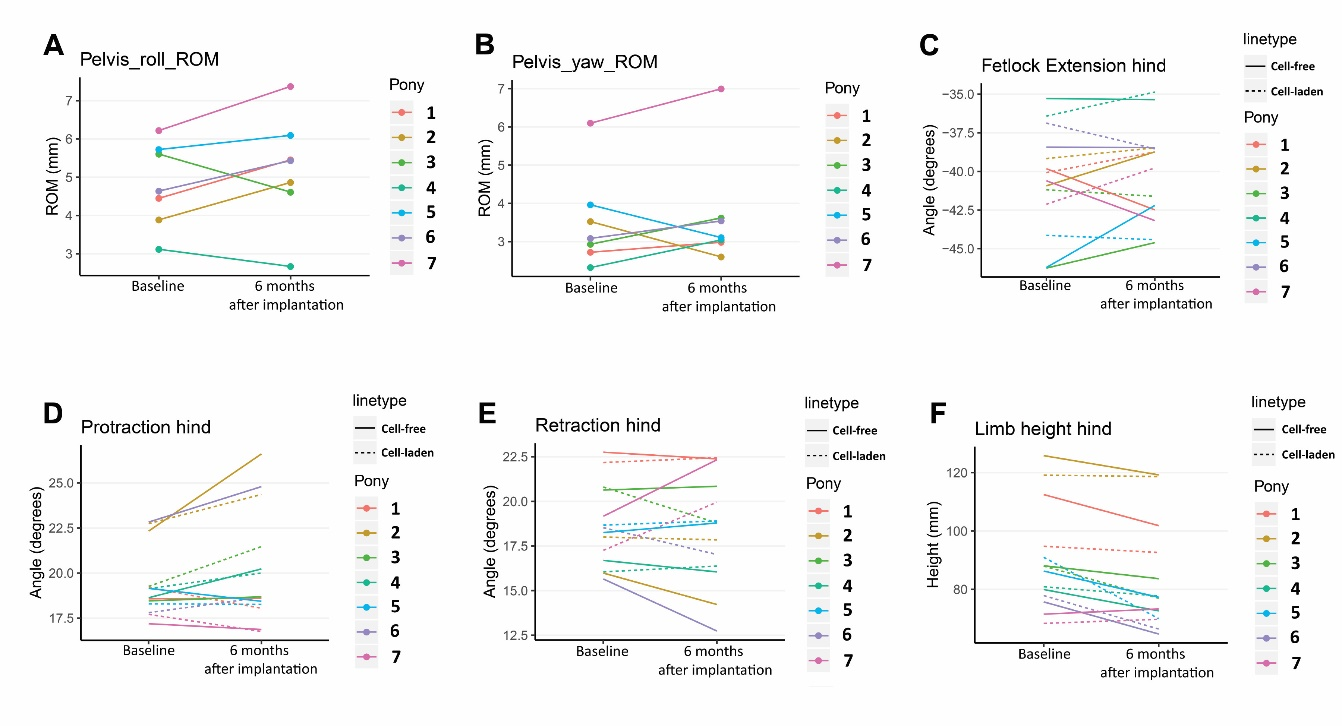
\includegraphics[width=\columnwidth+.8\fullwidthlen]{media/image12.jpg}
  \end{adjustwidth}
\begin{adjustwidth}{-.5\fullwidthlen}{}
\caption{\emph{Gait analysis: symmetry parameters.}
 Pelvis roll and yaw joint angles (A,B) showed no significant differences between baseline and 6 months after implantation and neither did the kinematic hind limb parameters (C, D, E) between baseline and 6 months after induction. Limb height of the hind limbs (F) decreased for both hindlimbs, but only significantly for the cell free group, though there was no difference in limb height between cell-laden and cell-free groups at 6 months after implementation.}
 \label{fig:sup1}
 \end{adjustwidth}
\end{figure*}



\begin{figure*}
      \captionsetup{width=\dimexpr \linewidth + \fullwidthlen\relax}

\begin{adjustwidth}{-\fullwidthlen}{}
 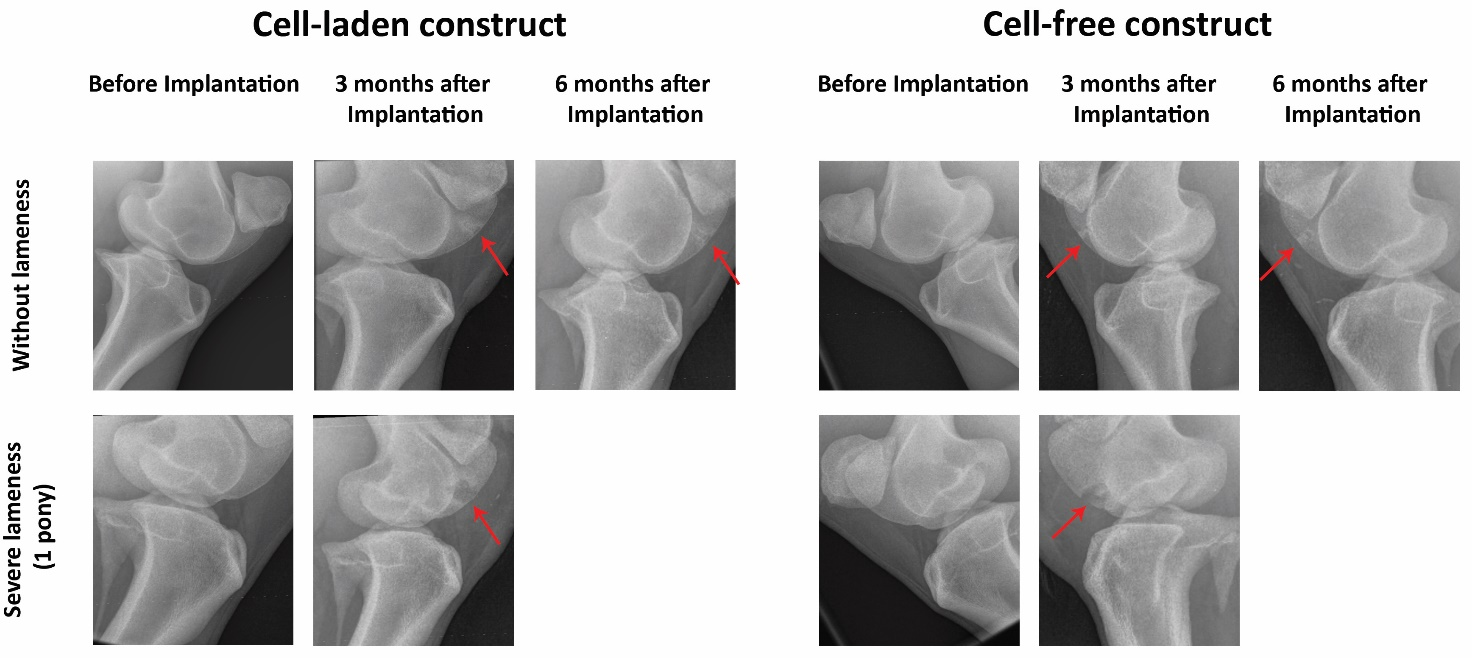
\includegraphics[width=\columnwidth+\fullwidthlen]{media/image13.jpg}
 \end{adjustwidth}
\begin{adjustwidth}{-.5\fullwidthlen}{}
\caption{\emph{Representative radiographic images (latero-medial and craniolateral-caudomedial oblique projections) of the stifle of ponies before implantation, 3 months after implantation and 6 months after implantation.}  Red arrows indicate the implantation sites. No radiographic abnormalities were noted in any of the ponies (1\textsuperscript{st} row), except for the pony that became severely lame at 10 weeks. In this animal extensive osteolysis was observed (2\textsuperscript{nd} row).}
\label{fig:sup2}
\end{adjustwidth}

\end{figure*}



\begin{figure}
\begin{adjustwidth}{-\fullwidthlen}{}
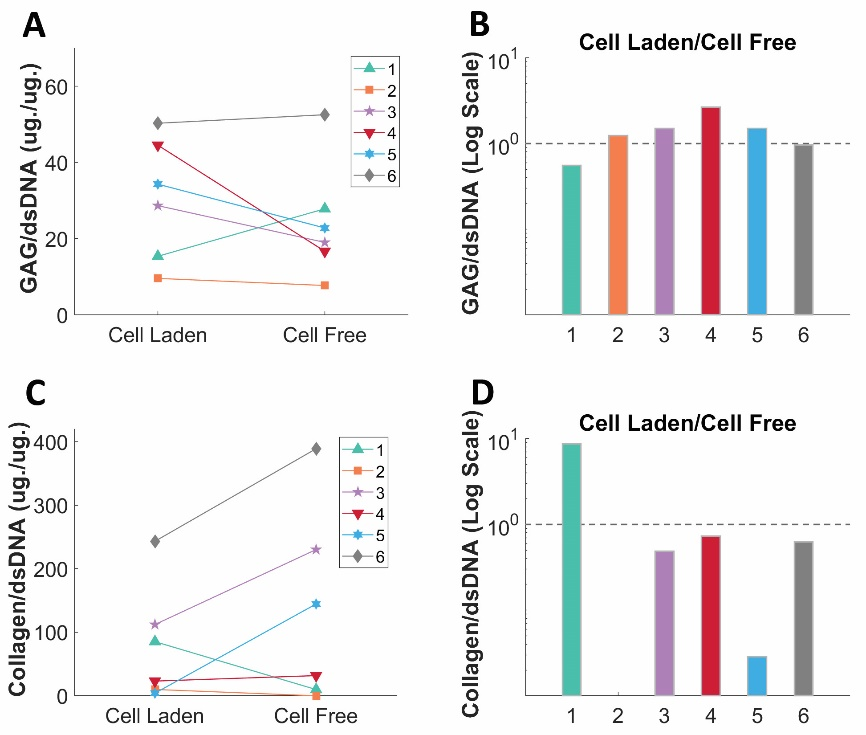
\includegraphics[width=\columnwidth]{media/image14.jpg}
\caption{\emph{Amount of GAG that was normalized with amount of DNA.}  Amount of GAG/DNA as absolute value (A) and as a ratio (B) in the individual animals. Amount of collagen/DNA as absolute value (C) and as a ratio (D) in the individual animals.}
\label{fig:sup3}
\end{adjustwidth}
\end{figure}


\begin{figure}
\begin{adjustwidth}{-\fullwidthlen}{}
 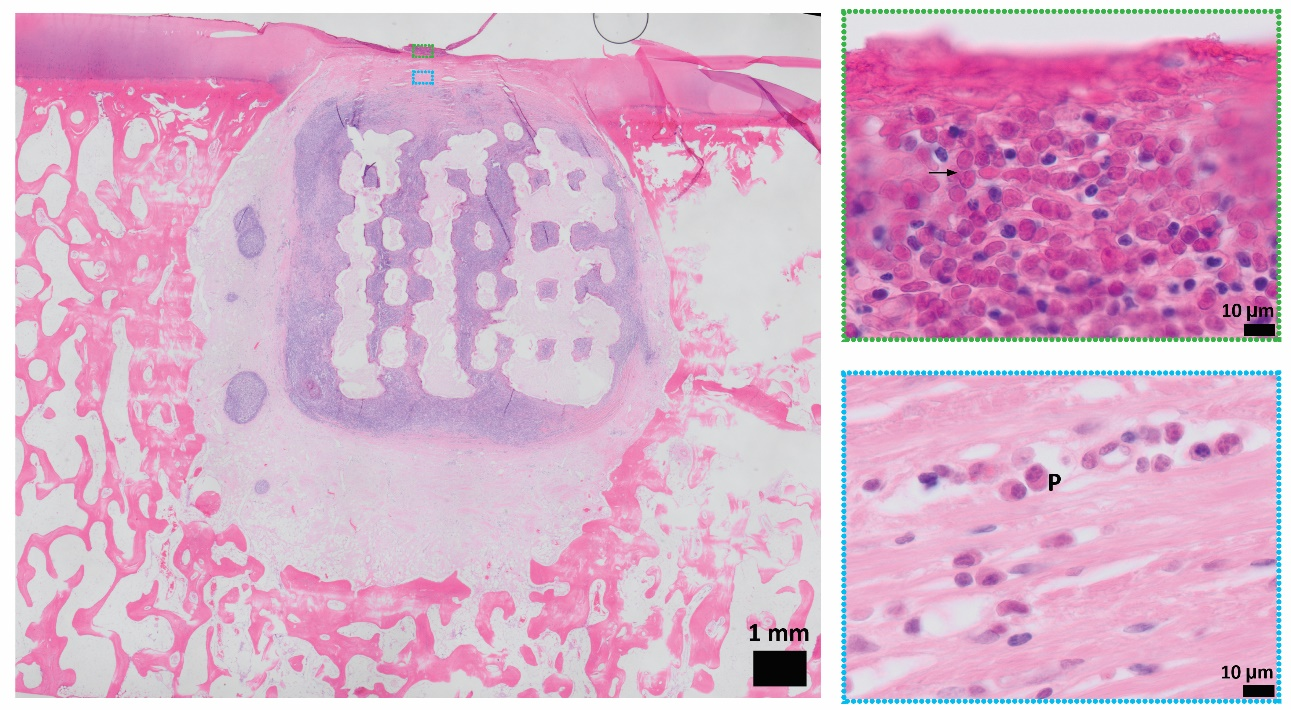
\includegraphics[width=.6\columnwidth]{media/image15.jpg}
\caption{\emph{Representative Hematoxylin-Eosin (H\&E) staining of 6-month harvested samples showing a degenerated and necrotic superficial layer at the surface of the chondral compartment featuring inflammatory cells.}  Black arrow indicates area of degenerated cells, P = plasma cells}
\end{adjustwidth}
\label{fig:sup4}
\end{figure}
\newpage
\twocolumn

\begin{figure}
\begin{adjustwidth}{-\fullwidthlen}{}
 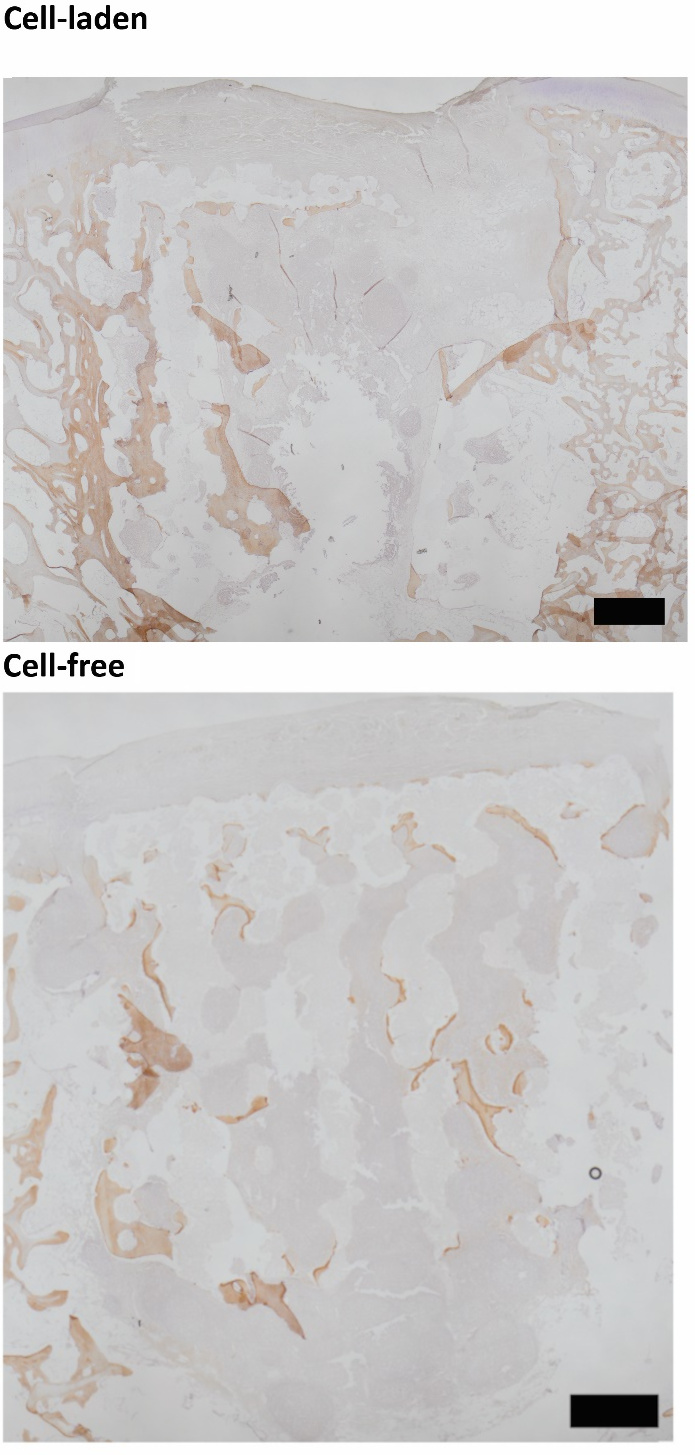
\includegraphics[width=.8\columnwidth+\fullwidthlen]{media/image16_1.jpg}
\caption{\emph{Representative immunohistochemistry of collagen type I staining of 6-month harvested samples from cell-laden and cell-free osteochondral structures}}
\label{fig:sup5}
\end{adjustwidth}
\end{figure}

\begin{figure}[t]
 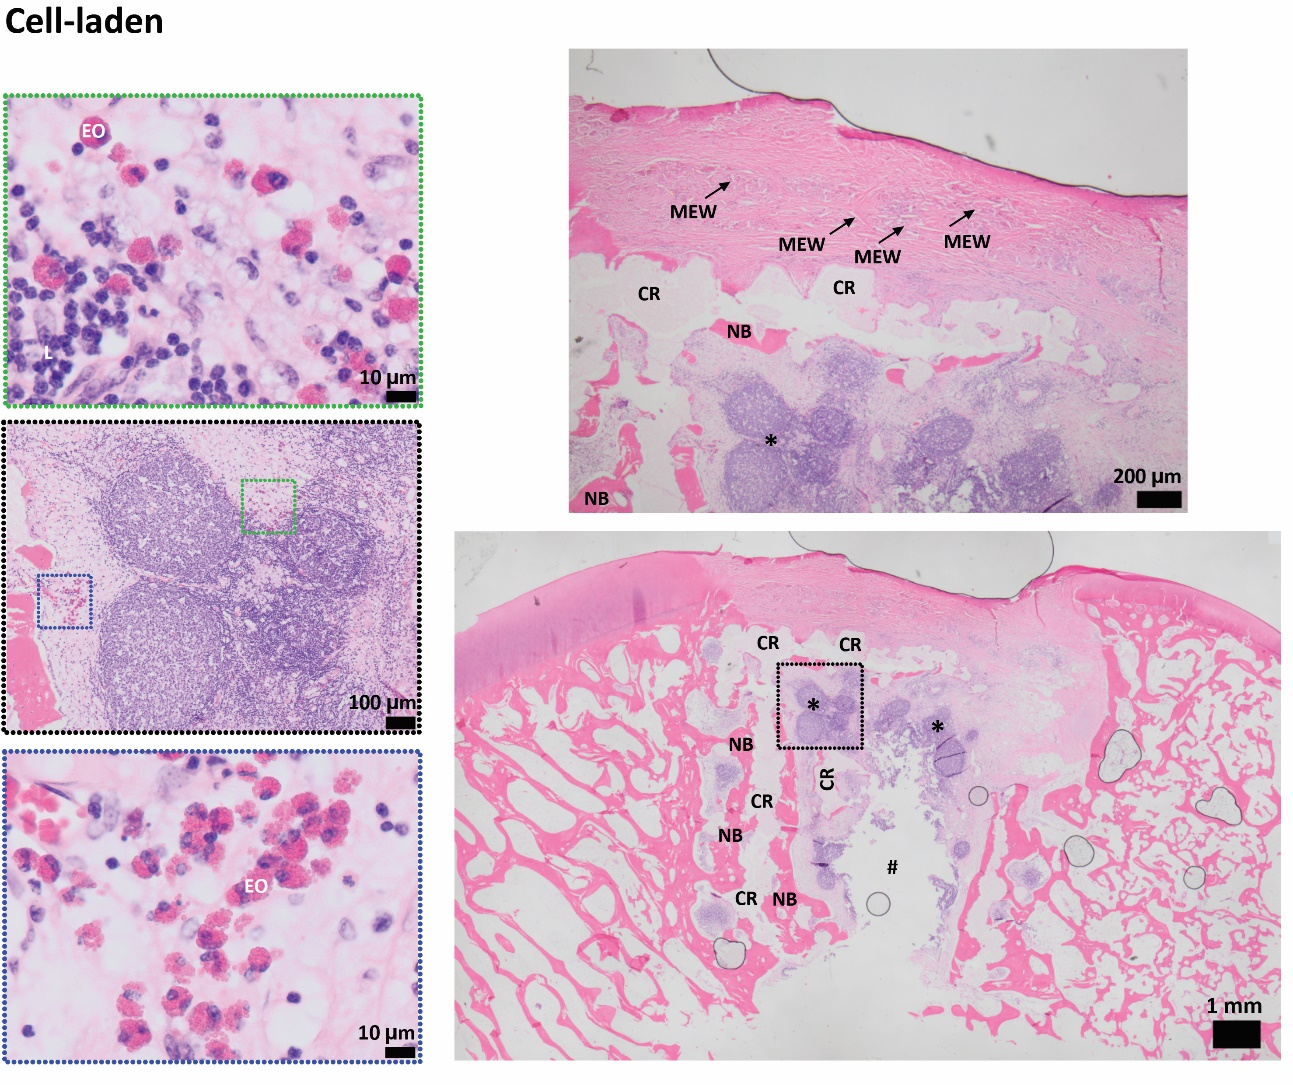
\includegraphics[width=1.02\columnwidth]{media/image17.jpg}
\caption{\emph{Representative Hematoxylin-Eosin (H\&E) staining of 6-month harvested samples from cell-laden osteochondral structures}  CR = Remaining ceramic, NB = Newly formed bone, MEW = pattern of PCL-microfibers, * = Multifocal foci of inflammatory reaction, \# = artifact from cutting, EO = Eosinophil, L = Lymphocyte}
\label{fig:sup6}\end{figure}


\begin{figure}[b]
 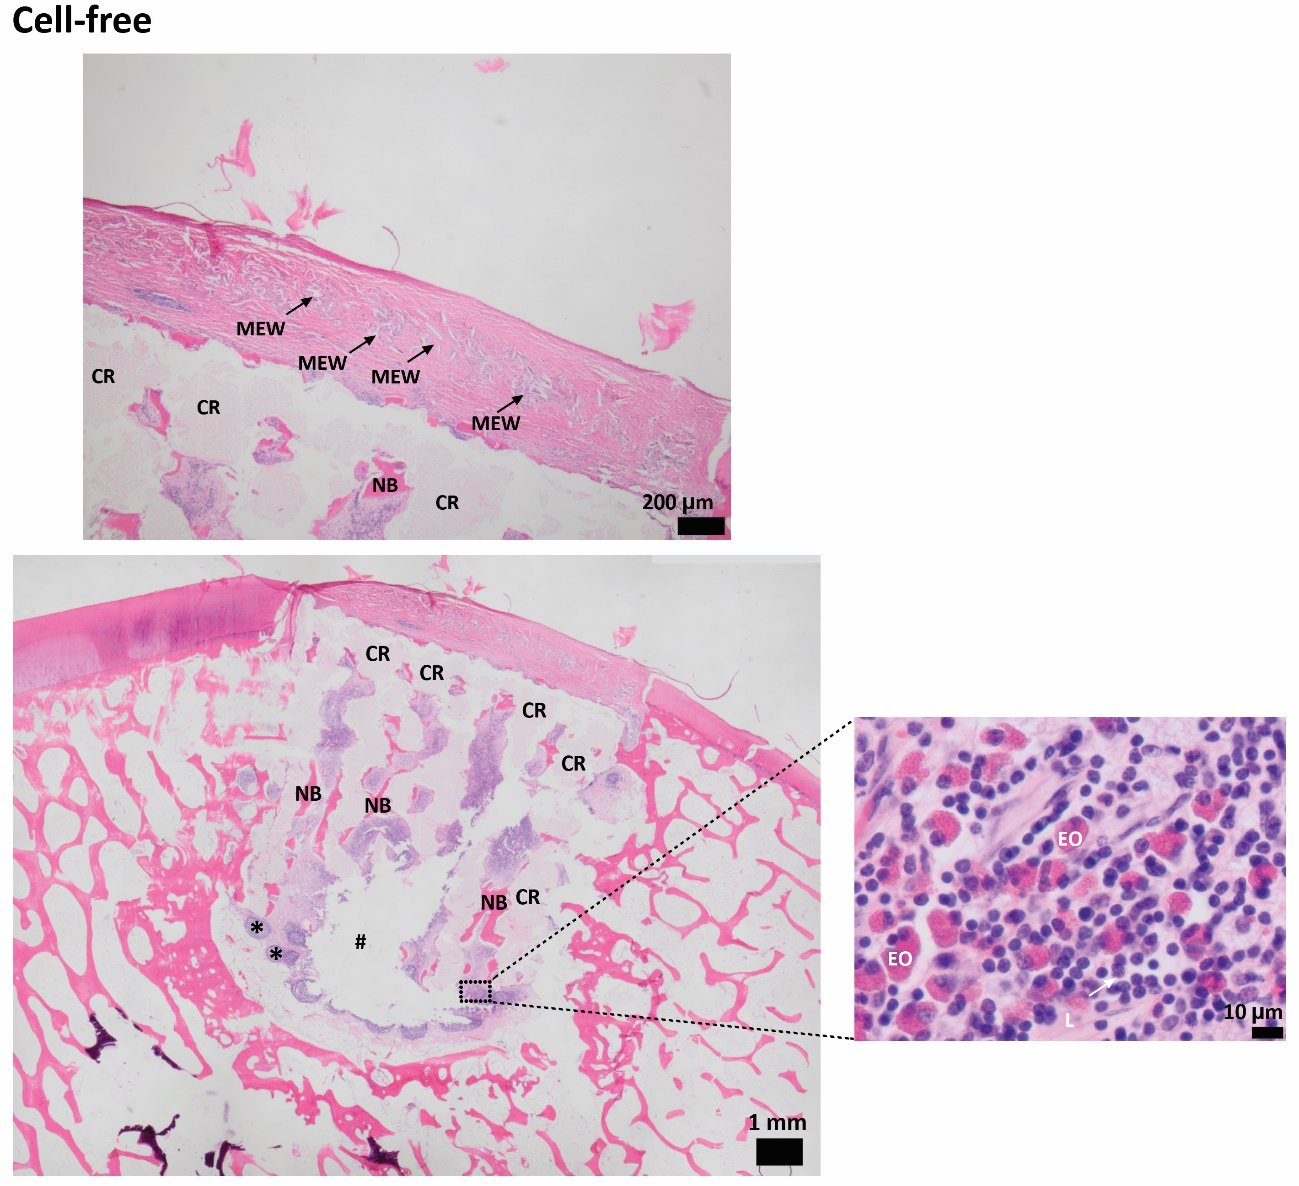
\includegraphics[width=\columnwidth]{media/image18.jpg}
\caption{\emph{Representative Hematoxylin-Eosin (H\&E) staining of 6-month harvested samples from cell-free osteochondral structures.}  CR = Remaining ceramic, NB = Newly formed bone, MEW = pattern of PCL-microfibers, * = Multifocal foci of inflammatory reaction, \# = artifact from cutting, EO = Eosinophil, L = Lymphocyte.}
\label{fig:sup7}\end{figure}


\end{document}
